\documentclass[10pt,twocolumn]{article}

% use the oxycomps style file
\usepackage{oxycomps}

% additional packages
\usepackage{pgfplots}
\pgfplotsset{compat=1.18}



% usage: \fixme[comments describing issue]{text to be fixed}
% define \fixme as not doing anything special
\newcommand{\fixme}[2][]{#2}
% overwrite it so it shows up as red
\renewcommand{\fixme}[2][]{\textcolor{red}{#2}}
% overwrite it again so related text shows as footnotes
%\renewcommand{\fixme}[2][]{\textcolor{red}{#2\footnote{#1}}}

% read references.bib for the bibtex data
\bibliography{references}

% include metadata in the generated pdf file
\pdfinfo{
    /Title (Magicode: An Educational Game to Teach Programming Fundamentals)
    /Author (Sammy Levy)
}

% UNCOMMENT TO RENDER WITHOUT ANY IMAGES
% \renewcommand{\includegraphics}[2][]{}

% set the title and author information
\title{\textit{Magicode:} \\ An Educational Game to Teach Programming Fundamentals}
\author{Sammy Levy}
\affiliation{Occidental College}
\email{slevy2@oxy.edu}

\begin{document}

\maketitle

\begin{abstract}
    This paper explores the design process and evaluation of \textit{Magicode}, an educational autobattler video game designed to teach the fundamentals of programming. Based in existing pedagogical theory, \textit{Magicode} uses a drag-and-drop programming language to implement a Game-Based Learning model designed to teach students who are new to code but familiar with video games. Through an iterative design process, user testing was conducted to develop the game and collect data on its effectiveness as an enjoyable experience and as a learning tool. Playtesters scored higher on an abstract programming knowledge quiz after playing the game, as well as reporting higher levels of confidence in programming ability.
\end{abstract}

\section{Introduction and Problem Context}
Since the earliest days of in-home computers, video games have been a staple of modern entertainment. Though the first games were often simple in scope, some standout games from even the early 1970s provided players with engaging, replayable, and simply fun gameplay systems. In particular, \textit{The Oregon Trail}, released in 1971 by the Minnesota Educational Computing Consortium (MECC) \cite{oregon-trail-video}, grew to become a household name due to the game’s simplicity and educational aspects. Though this initial version was a text-based version of the game played solely in the command line, updated versions of the game continually developed by MECC included graphics and minigames to further engage players \cite{oregon-trail-archived}.

What made \textit{The Oregon Trail} educational was its basis in maintaining historical accuracy. This is implemented in gameplay through its brutal difficulty; in maintaining historical accuracy, it forces players to manage a tight budget, food rationing, and deaths of family members. Despite its harshness, however, the game was intended for a younger player base. Through gameplay, elementary- and middle school-aged children could learn and apply the basics of math, history, and geography that they also use in the classroom.

I grew up playing the Oregon Trail, among other educational games, as a productive outlet to explore my passion for video games. As both of my parents are educators who have worked on developing educational games and software in the past, there is little guess work required to see where my passion stems from. For my Senior Comprehensive Project (Comps), I sought to combine my love of video games and game design with my work as an Education minor to develop an educational game rooted in the foundational theories that I have learned in my time here at Occidental.

My game, \textit{Magicode}, is an educational autobattler video game designed to teach programming fundamentals. As described by Edsger W. Dijkstra in the late 1980s, teaching people how to code is a notoriously difficult task due to a concept he called “radical novelty” \cite{dijkstra-difficulty}, defined as a new idea that cannot be adequately conceptualized in terms of preexisting knowledge and vocabulary. Thus, radically novel education practices are necessary to effectively teach these concepts. This is the space in which Magicode fits, using the oft-overlooked video game medium, especially the newer autobattler genre \cite{autobattler-genre}, as a radical teaching tool. My goal is to provide players with a fun and engaging educational experience from which they can take away transferable skills as they further their Computer Science education.

\begin{figure}
    \centering
    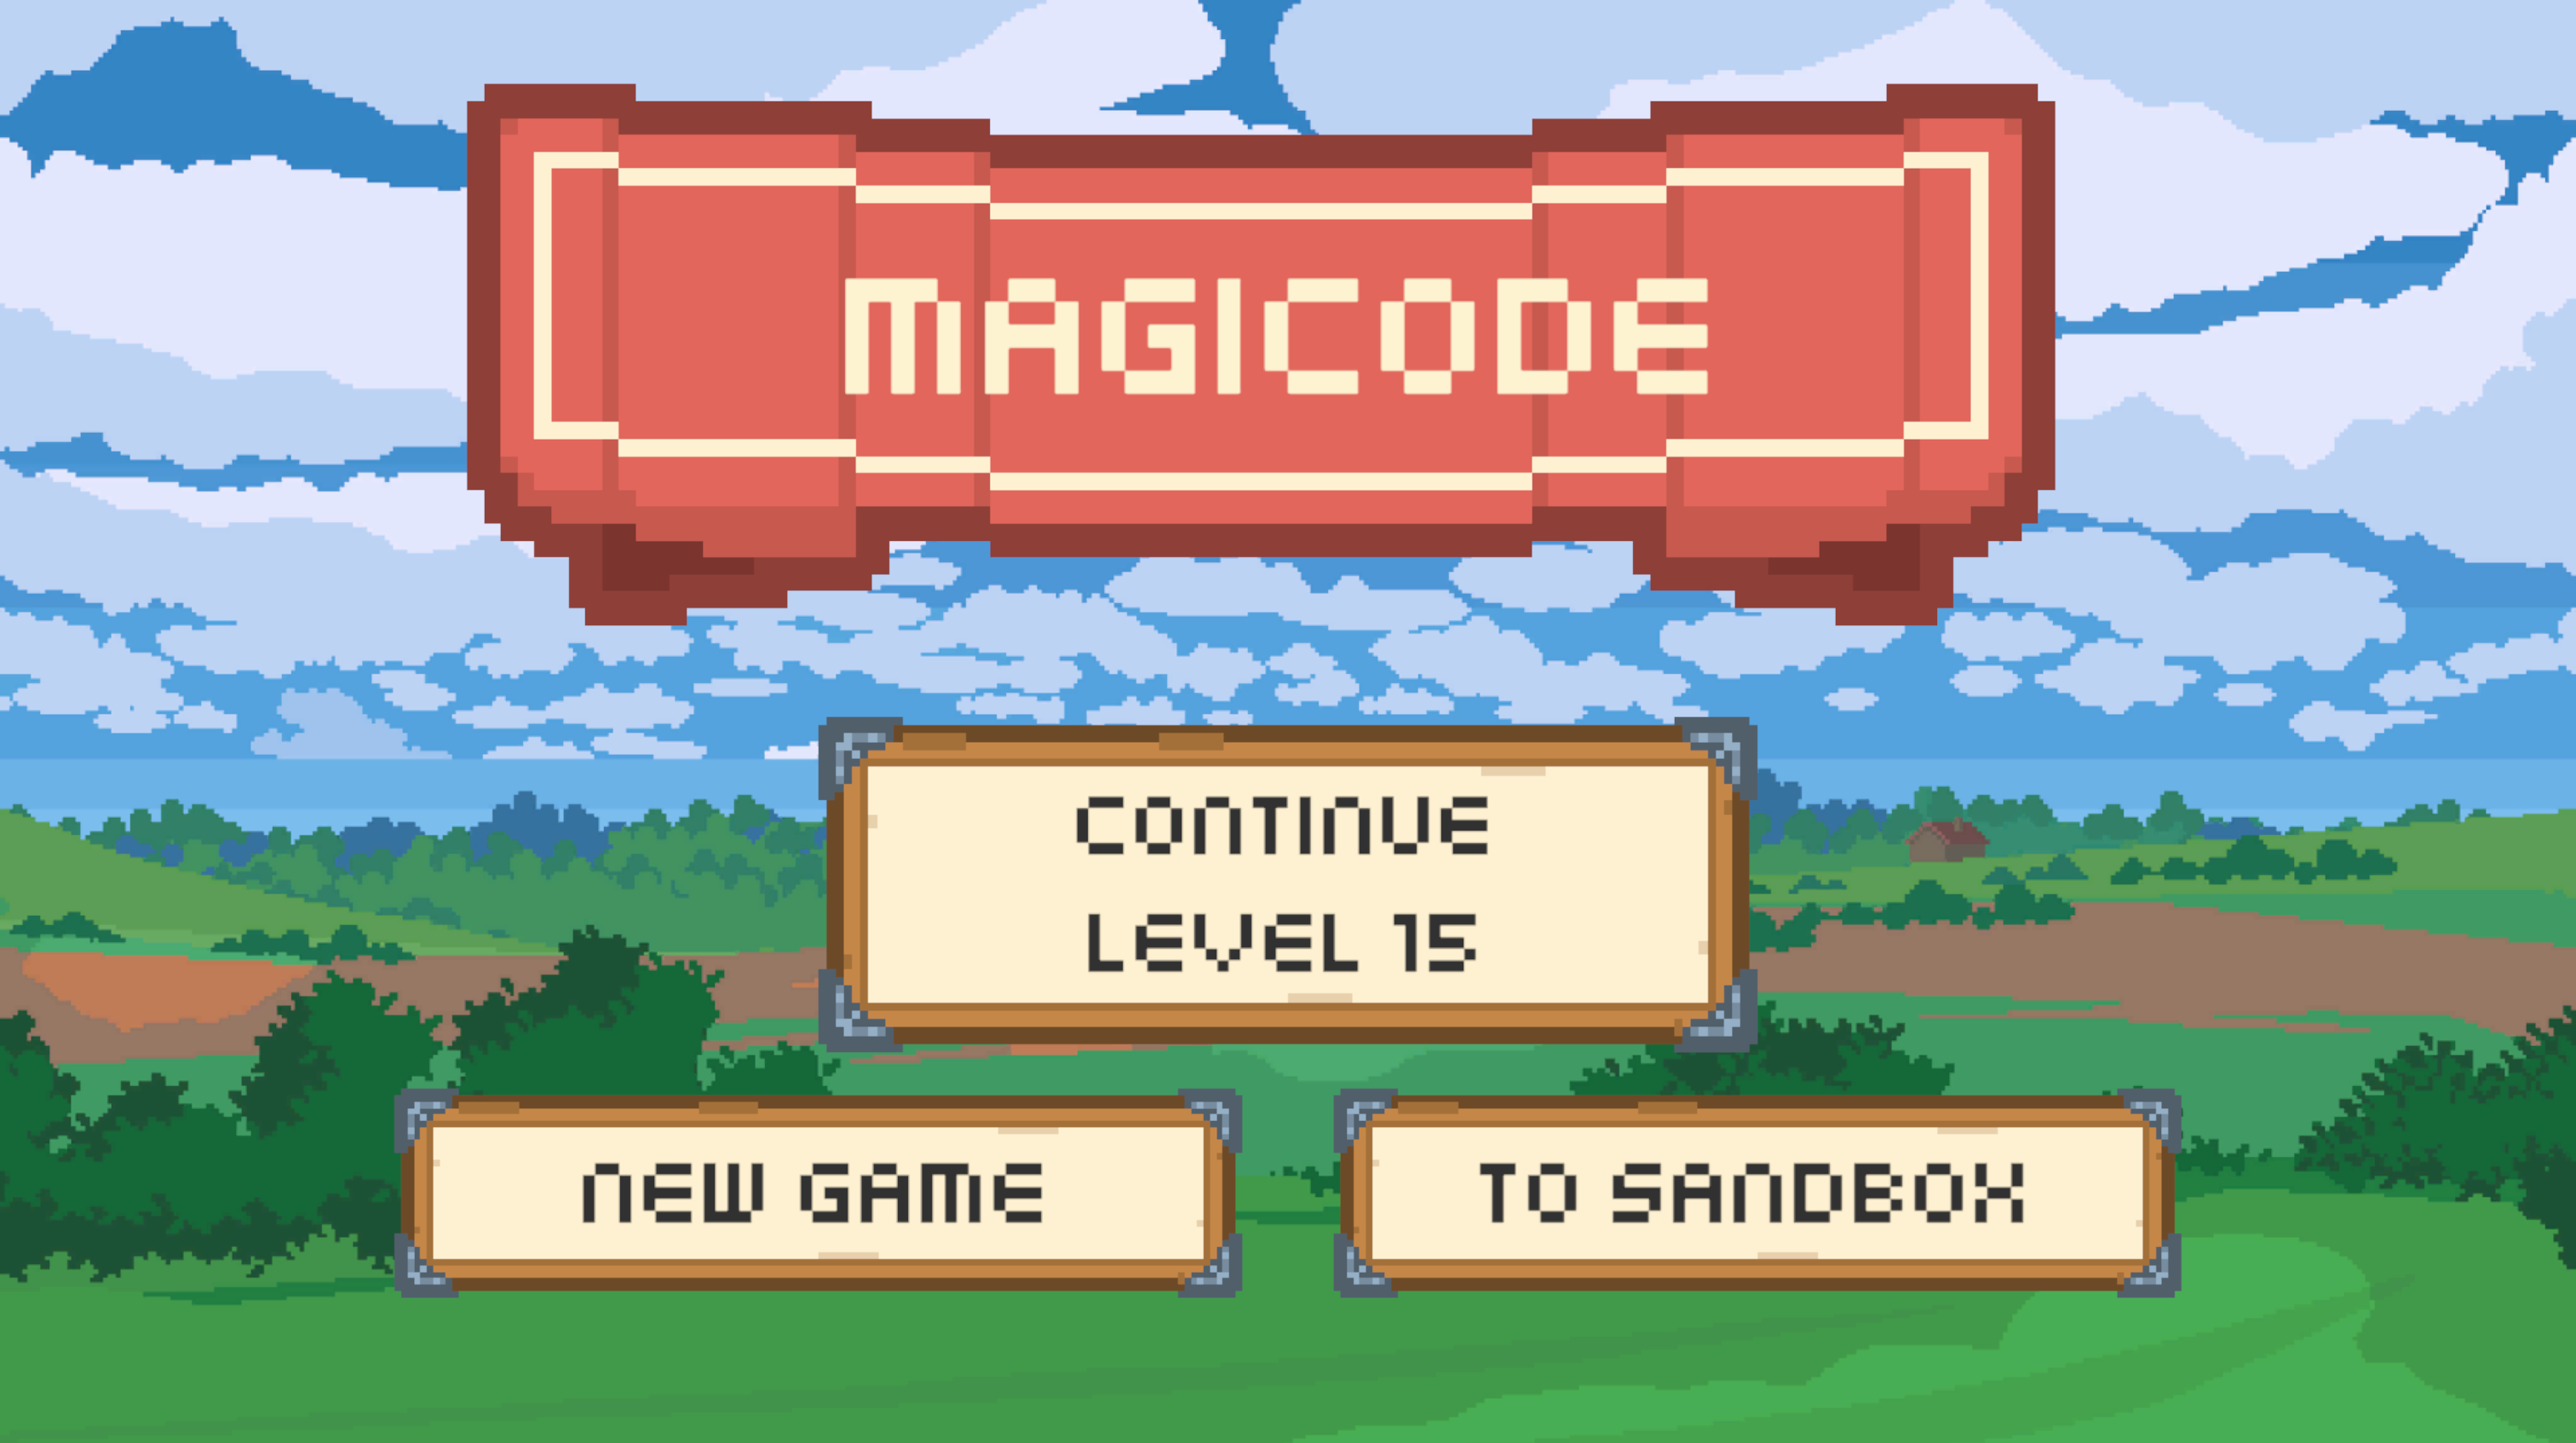
\includegraphics[width=\linewidth]{images/screenshots/main_menu.png}
    \caption{The main menu screen of \textit{Magicode}.}
    \label{fig:main-menu}
\end{figure}

The target audiences of \textit{Magicode} are high school and college aged students who are familiar with video games, but have minimal prior coding experience, which is not a demographic often catered to by educational games. Given that of this age in the last generation and beyond have grown up with exposure to this medium, my project is in a unique position to fill a void and help students find the joy in learning how to code.


\section{Technical Background}
I developed \textit{Magicode} using the Unity game engine with scripting in C\# \cite{unity-website}. The design of the game will be explored further in section 4, but the technical aspects of the game’s design can be broken down into two components: building an autobattler game and building a simple, drag-and-drop coding language. These elements are used together to create the core gameplay loop. This section will also explore an educational framework for curriculum design.

\subsection{Autobattlers}
The Autobattler is a new genre of game, popularized by games like \textit{Autochess} \cite{autochess-steam} and \textit{Teamfight Tactics} \cite{tft}. These are both competitive, online multiplayer games in which players compete against each other in multiple rounds by choosing characters from a shared pool, upgrading them, and placing them on a battlefield to fight each other automatically. Though this may at first seem like an unengaging system, the appeal of autobattlers comes from the strategy needed to win each fight. Creative character placement, strategic synergizing of character abilities, and learning how to counter opposing strategies are the core of what makes the genre engaging.

With this in mind, it is not a stretch to say that autobattlers are not action games, but instead competitive puzzle games. Using learnable (and therefore predictable) algorithms to calculate turn order, attack effects, and character movement, players must strategize to solve the puzzle of defeating their opponent in each round of the game. \textit{Magicode} leans heavily into the puzzle aspect of the autobattler genre as a single-player game. Instead of competing with a real opponent, players fight against predetermined groups of enemies that are designed and positioned precisely to require a certain solution (or multiple solutions) to complete their respective level. Players also design characters instead of selecting from a predetermined pool is also a key difference, adding an additional strategic dimension wherein players must design characters that work together effectively.

Aside from these differences, \textit{Magicode} is played like any other autobattler by placing warriors on the battlefield and watching them fight automatically. To design effective solutions for each level, the player must learn how their enemies behave and implement newly introduced mechanics. Without the inclusion of multiplayer features, the player focuses on learning key concepts and optimizing solutions instead of competition.

\subsection{Language}
The other phase of \textit{Magicode}’s gameplay is based in a visual coding language. Though the game itself is programmed in C\#, my intention is to give novice coders an opportunity to use fundamental programming concepts without having to worry about the syntax of a full, text-based programming language. Visual programming has historically been used to teach programming fundamentals to beginners, as well as provide an easier way for non-programmers (e.g. artists) in a team-based project to have more hands-on influence \cite{visual-oop}. Though there are multiple styles of visual programming, \textit{Magicode} implements drag-and-drop coding, a system where simple blocks of code are presented to the user, and they can be dragged around the screen in order to form scripts for a given object. The Scratch programming language is an example of this, where its easy-to-learn, block-based coding system serves as an introduction to code for many aspiring computer science students \cite{scratch-website}.

\begin{figure}
    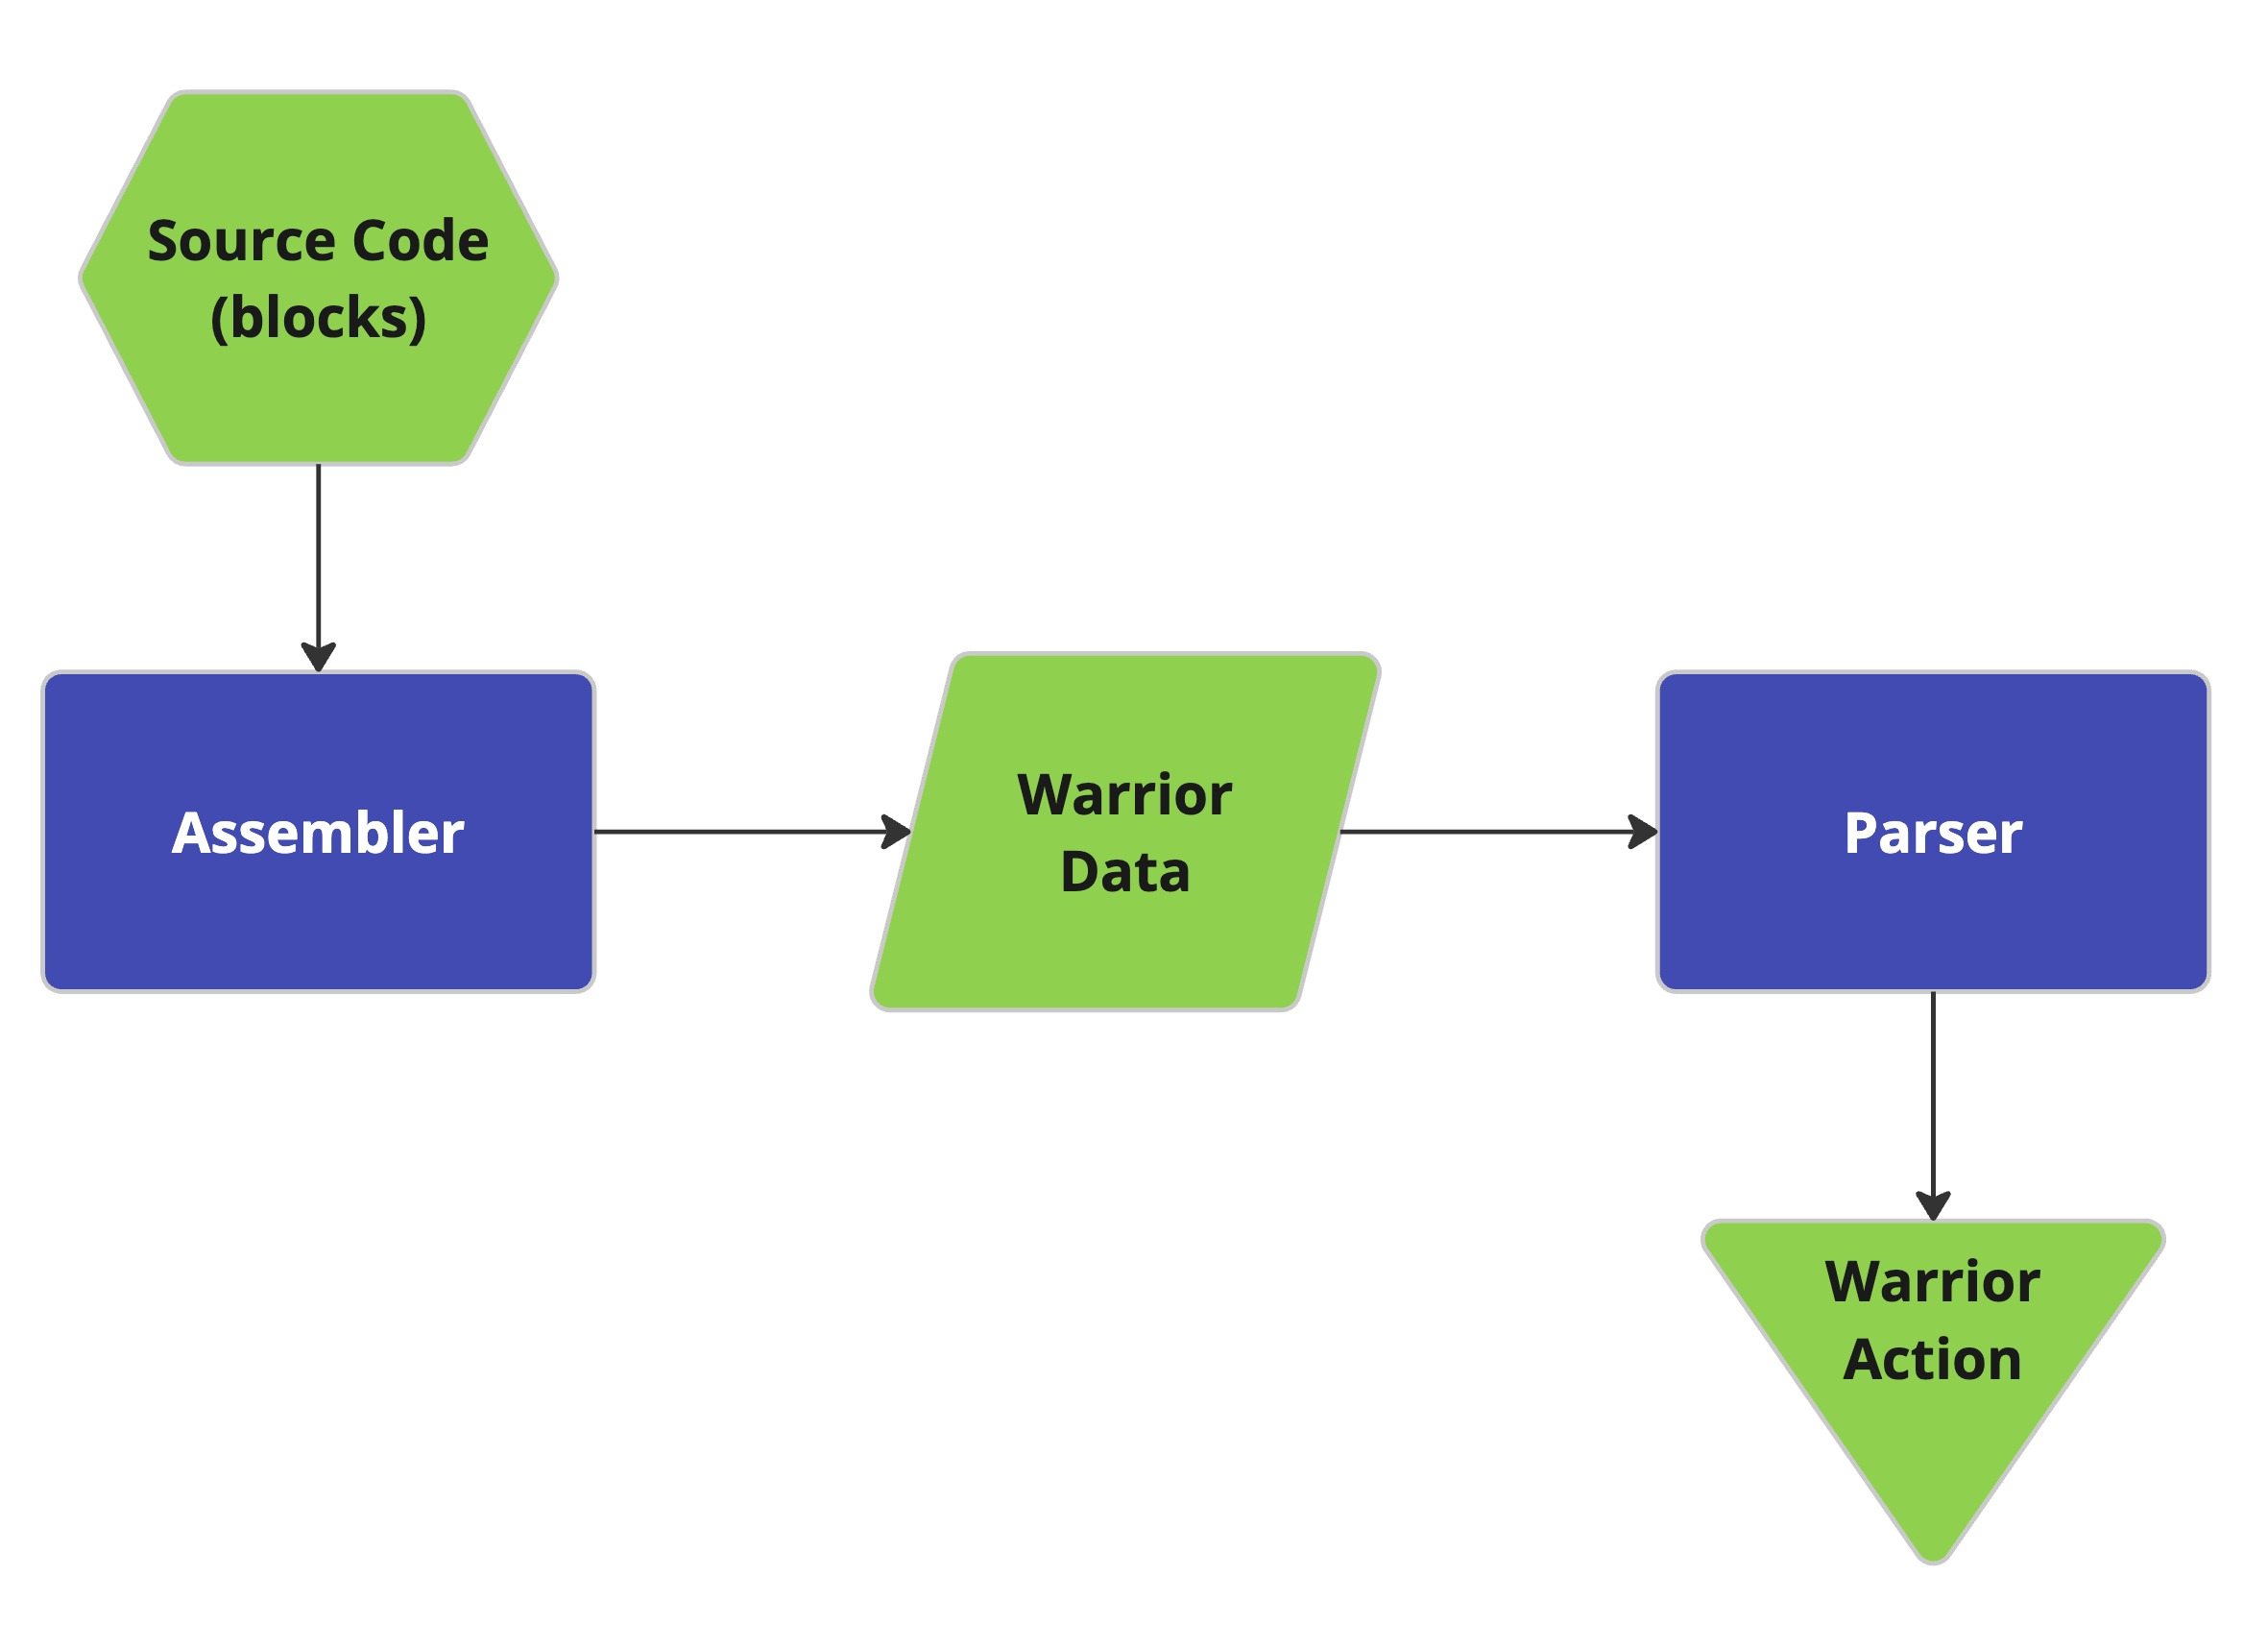
\includegraphics[width=\linewidth]{images/compiler.jpg}
    \caption{Code is assembled and parsed from blocks into warrior action.}
    \label{fig:compiler-diagram}
\end{figure}


Though my language is inspired by Scratch, it is not nearly as wide in scope. New programming languages are developed to fill gaps or fit specific needs; for example, Python was initially created as an easier way to interact with the Amoeba operating system, though its design philosophy has grown to become a language that is easy to learn yet robust enough to handle large scale projects \cite{why-python}. The reach of my language does not extend beyond the scope of gameplay, thus the player will not need the freedom to program anything unrelated to the game. Rather, each programmable warrior in the game will have a discrete set of functions (e.g. “move”, “use weapon”) that the player can modify using code blocks.


Designing a new language often involves building a compiler or an interpreter, among some other key details required for the computer to understand the language. In the simplified language that I created, there are two key steps for code interpretation. As seen in Figure \ref{fig:compiler-diagram}, the assembler and the parser translate player-written code into character actions in game. Firstly, the assembler reads each code block and converts its data into object code, converting high-level code blocks into a sequence of IDs and values that are not readable to the player \cite{assembly-textbook}. This object code is read by the parser during gameplay, turning each instruction into character actions by executing atomic functions using stored values as arguments \cite{compiler-textbook}. All conditionals and loops store instructions when assembled: pointers to their beginnings and ends that tell the parser which instructions to jump to in the sequence, based on successful and unsuccessful condition matches. To prevent runtime errors, all code blocks have default values and behaviors if the player makes a critical mistake.

\subsection{Bloom's Taxonomy of Educational Objectives}
\textit{Bloom’s Taxonomy of Educational Objectives} (BTEO) is a cumulative framework for curriculum development and analysis, authored by Benjamin Bloom in 1956 \cite{bloom-taxonomy}. The objectives are as follows:

\begin{itemize}
    \item Knowledge
    \item Comprehension
    \item Application
    \item Analysis
    \item Synthesis
    \item Evaluation
\end{itemize}

In a well-constructed curriculum for any subject, each of these objectives build on one another. First, a basis of \textit{knowledge} in the subject material is established. \textit{Comprehension} comes from the ability to connect individual elements of this knowledge together, and \textit{application} expands this skill by connecting the knowledge to previous knowledge. \textit{Analysis} and \textit{synthesis} see the deconstruction and reconstruction of new scenarios using applied knowledge. Finally, the skill of \textit{evaluation} stems from full understanding of the subject material, allowing for critique and stronger critical analysis of future content within the subject area. 

As an educational tool, \textit{Magicode}’s level structure is designed to implement BTEO both individually and sequentially. Each level introduces players to new mechanics and requires experimentation to learn how they interact with each other and previous mechanics. From there, players must analyze the level, synthesize a solution, and evaluate their success or failure to progress. In sequence, each level introduces new mechanics with increasing complexity, and success throughout the game requires the development of skills within these objectives. Section 6 contains an analysis of the outcomes of BTEO within the game based on player feedback. 

Notably, the taxonomy was revised in 2001, renaming curriculum goals to be more action-oriented and swapping the final two objectives \cite{revised-taxonomy}. However, \textit{Magicode}’s educational objectives are designed using the original taxonomy, as I felt that the initial ordering better reflects the cycle of experimentation players engage with during gameplay. BTEO has historically been applied to all subjects, and its use within Computer Science curriculum is no exception \cite{teaching-oop}.


\section{Prior Work}
Coding games can generally be split into one of two categories: \textit{Pure Code} games, which focus on teaching literal language usage, and \textit{Optimization} games, which follow a more abstract approach to coding through puzzles. Since \textit{Magicode} fits somewhere in the gray area between these categories, this section will explore the benefits of both types of coding games. Here, I also explore the educational foundations of Game-Based Learning, and how it is integrated at the core of my game.

\subsection{Coding Games}
\textit{Pure Code} games, which I define as games that use a real coding language as a core part of their gameplay, serve as one part of the design framework of \textit{Magicode}. These games do not necessarily require much UI in order to play the game, as the vast majority of “gameplay” happens through the coding process. \textit{Robocode}, a game created in the early 2000s that is still operational today, allows players to design and program virtual robots that fight other robots designed by other players online \cite{robocode}. Its gameplay requires the use of an external text editor or IDE where the robot’s backend code is written in Java using a custom API created by the game’s developers. After a robot’s creation, it can be entered into a battle, which appears as a new window displaying a top-down view of all robots. Battles can either play out automatically or be influenced by the player’s programmed control scheme. While there are external resources available to learn how to both play the game and optimize a robot’s code, \textit{Robocode} itself includes neither an explicit tutorial nor a system of progression that teaches the player how to code.

A similar project that does include an educational structure is \textit{CodeCombat}, another Pure Code game \cite{code-combat}. \textit{CodeCombat} guides players through a series of levels set in a fantasy world that teach the fundamentals of programming in a wide variety of languages. As compared to \textit{Robocode}, this game provides a much more structured experience. In Javascript, Python, or other popular programming languages, players are asked to use logic and write functions to define the movement and behavior of their character. While \textit{Magicode} uses a visual programming language to dampen the learning curve, the concept of programming objects to fight automatically as seen in \textit{Robocode} and \textit{CodeCombat} is part of the core gameplay loop.

\textit{Optimization} games, on the other hand, are puzzle games that use programming in a simplified language as a core gameplay mechanic. Often, players receive a score at the end of each level that conveys how “optimal” their solution was in terms of time and space complexity, among other game-specific metrics. \textit{Human Resource Machine} \cite{human-resource-machine-steam} and \textit{Opus Magnum} \cite{opus-magnum-steam} are two such critically acclaimed games. The former sees the player using an assembly-like visual programming language to instruct corporate characters to move specific blocks from one location to another in each level. The game’s language is an abstraction of key concepts needed to understand assembly code; for example, later levels require the use of registers, jumps, and conditional statements to succeed. The player does not directly interact with the objects and characters in the level; they can only manipulate them through code.

\textit{Opus Magnum} uses both forms of player interaction: in this steampunk, alchemy-themed game, players must both design and program machines that move, transform, and combine objects to complete each level’s objective. The design aspect involves placing mechanical arms (and other useful contraptions) around a hexagonal grid to will pick up, modify, and move elements to achieve a designated goal. In terms of programming, players choose from a list of thirteen function blocks (e.g. “pick up”, “extend”, “rotate”) to define a linear set of instructions for each arm to follow, which play out for each arm simultaneously with the press of a button. Success in \textit{Opus Magnum} requires an understanding of both the engineering and programming concepts.

\begin{figure}
    \centering
    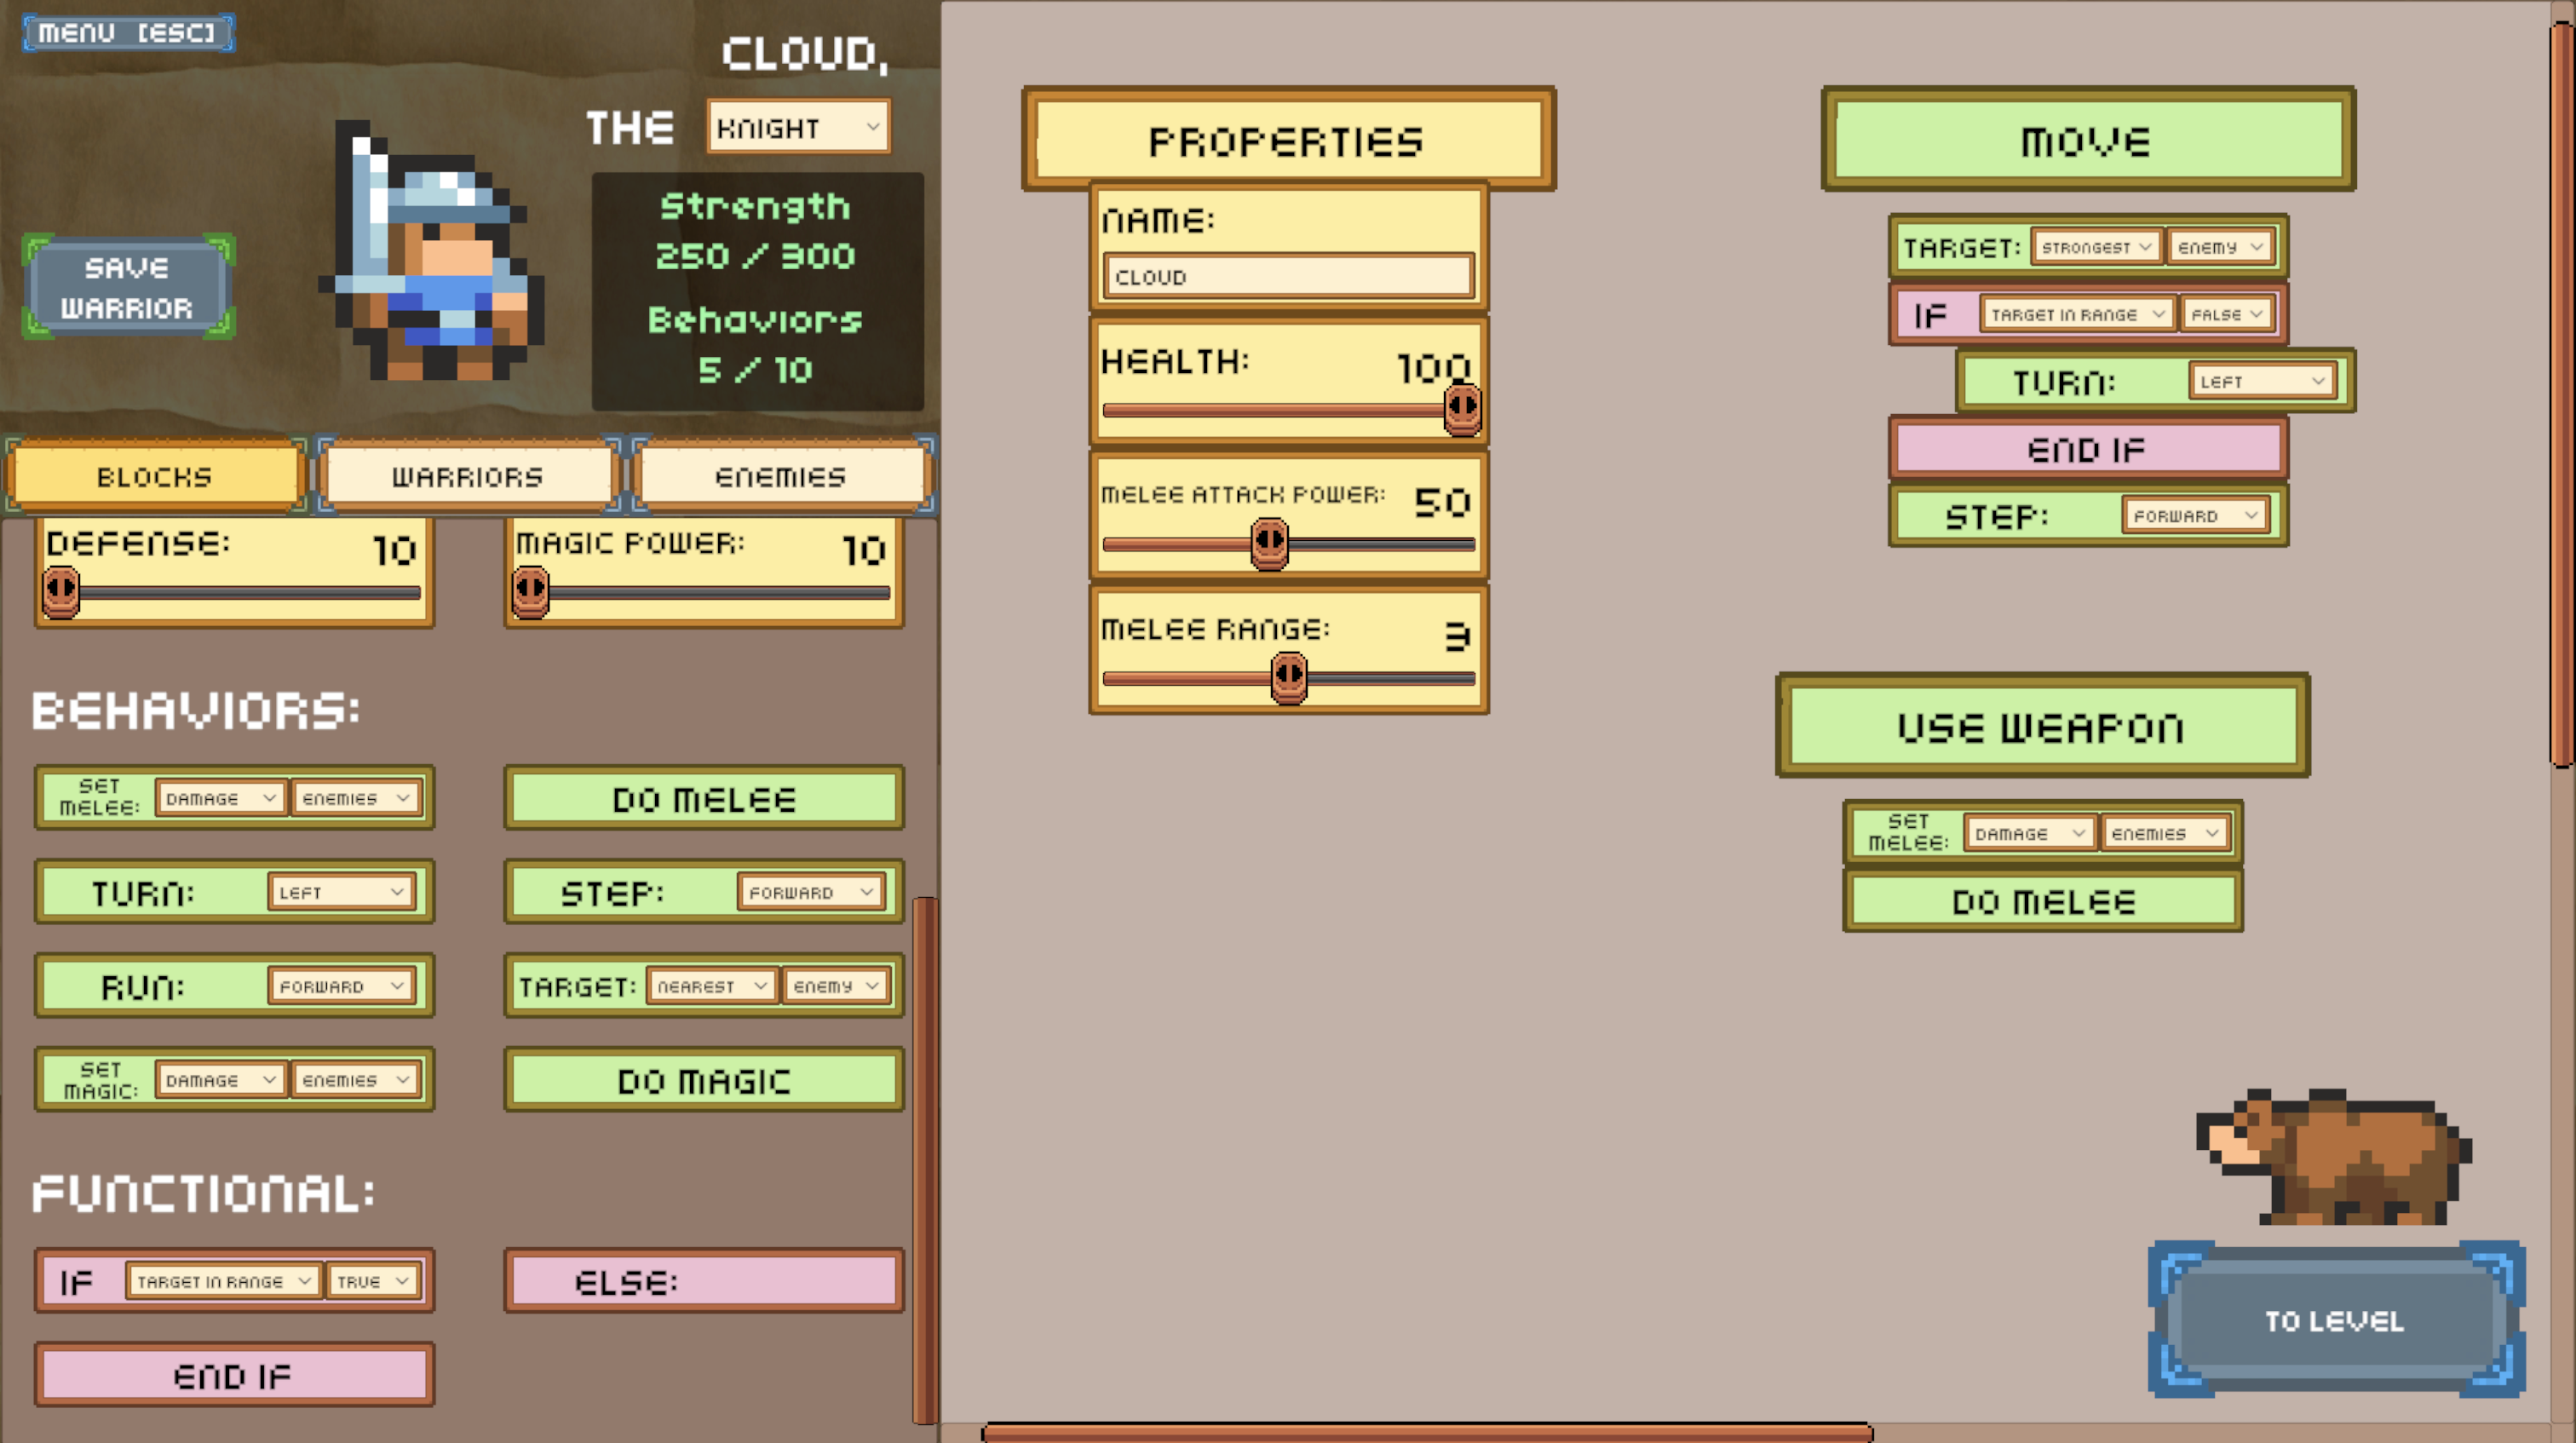
\includegraphics[width=\linewidth]{images/screenshots/cloud_editor.png}
    \caption{The code editor with a simple warrior.}
    \label{fig:code-editor-screenshot}
\end{figure}

My game takes inspiration from both of these games in its design. The assembly-like structure of Human Resource Machine’s programming language inspired \textit{Magicode}’s conditional structures and aided with simplifying backend development. Opus Magnum’s deceptively simple level design that leaves space for a variety of solutions that all require usage of new mechanics, or twists on old mechanics, was taken into consideration when designing enemies and level layouts. The abstracted yet conceptually solid programming languages seen in Optimization games inspired \textit{Magicode}'s drag-and-drop programming language. This, in combination with the Game-Based Learning framework of Pure Code games, leads to a fun, intellectual challenge.

\subsection{Game-Based Learning}
The two common frameworks for introducing games into the classroom are Gamification and Game-Based Learning (GBL), the latter of which is the core of my project. Whereas gamification involves applying game-like elements to classroom lectures and activities, GBL uses games themselves as learning tools, such as stock market simulations and physics-based games \cite{gbl-waterloo}. From a very young age, children use play to bridge the gaps between abstract concepts and their physical reality; by intentionally harnessing the way we seek out play, educational games increase both the amount of content learned and the motivation to learn \cite{foundations-gbl}. This can be seen more concretely through Vygotsky’s (1978) Zone of Proximal Development \cite{vygotsky}, a commonly cited educational theory that identifies that a transitional state between a student’s comfort zone and discomfort zone is where the greatest amount of learning occurs. This middle area sees students applying what they know in new situations or introducing new concepts into familiar situations. GBL presents the students with the latter, providing a playful, familiar environment in which new concepts can be introduced with low stakes.

\begin{figure}
    \centering
    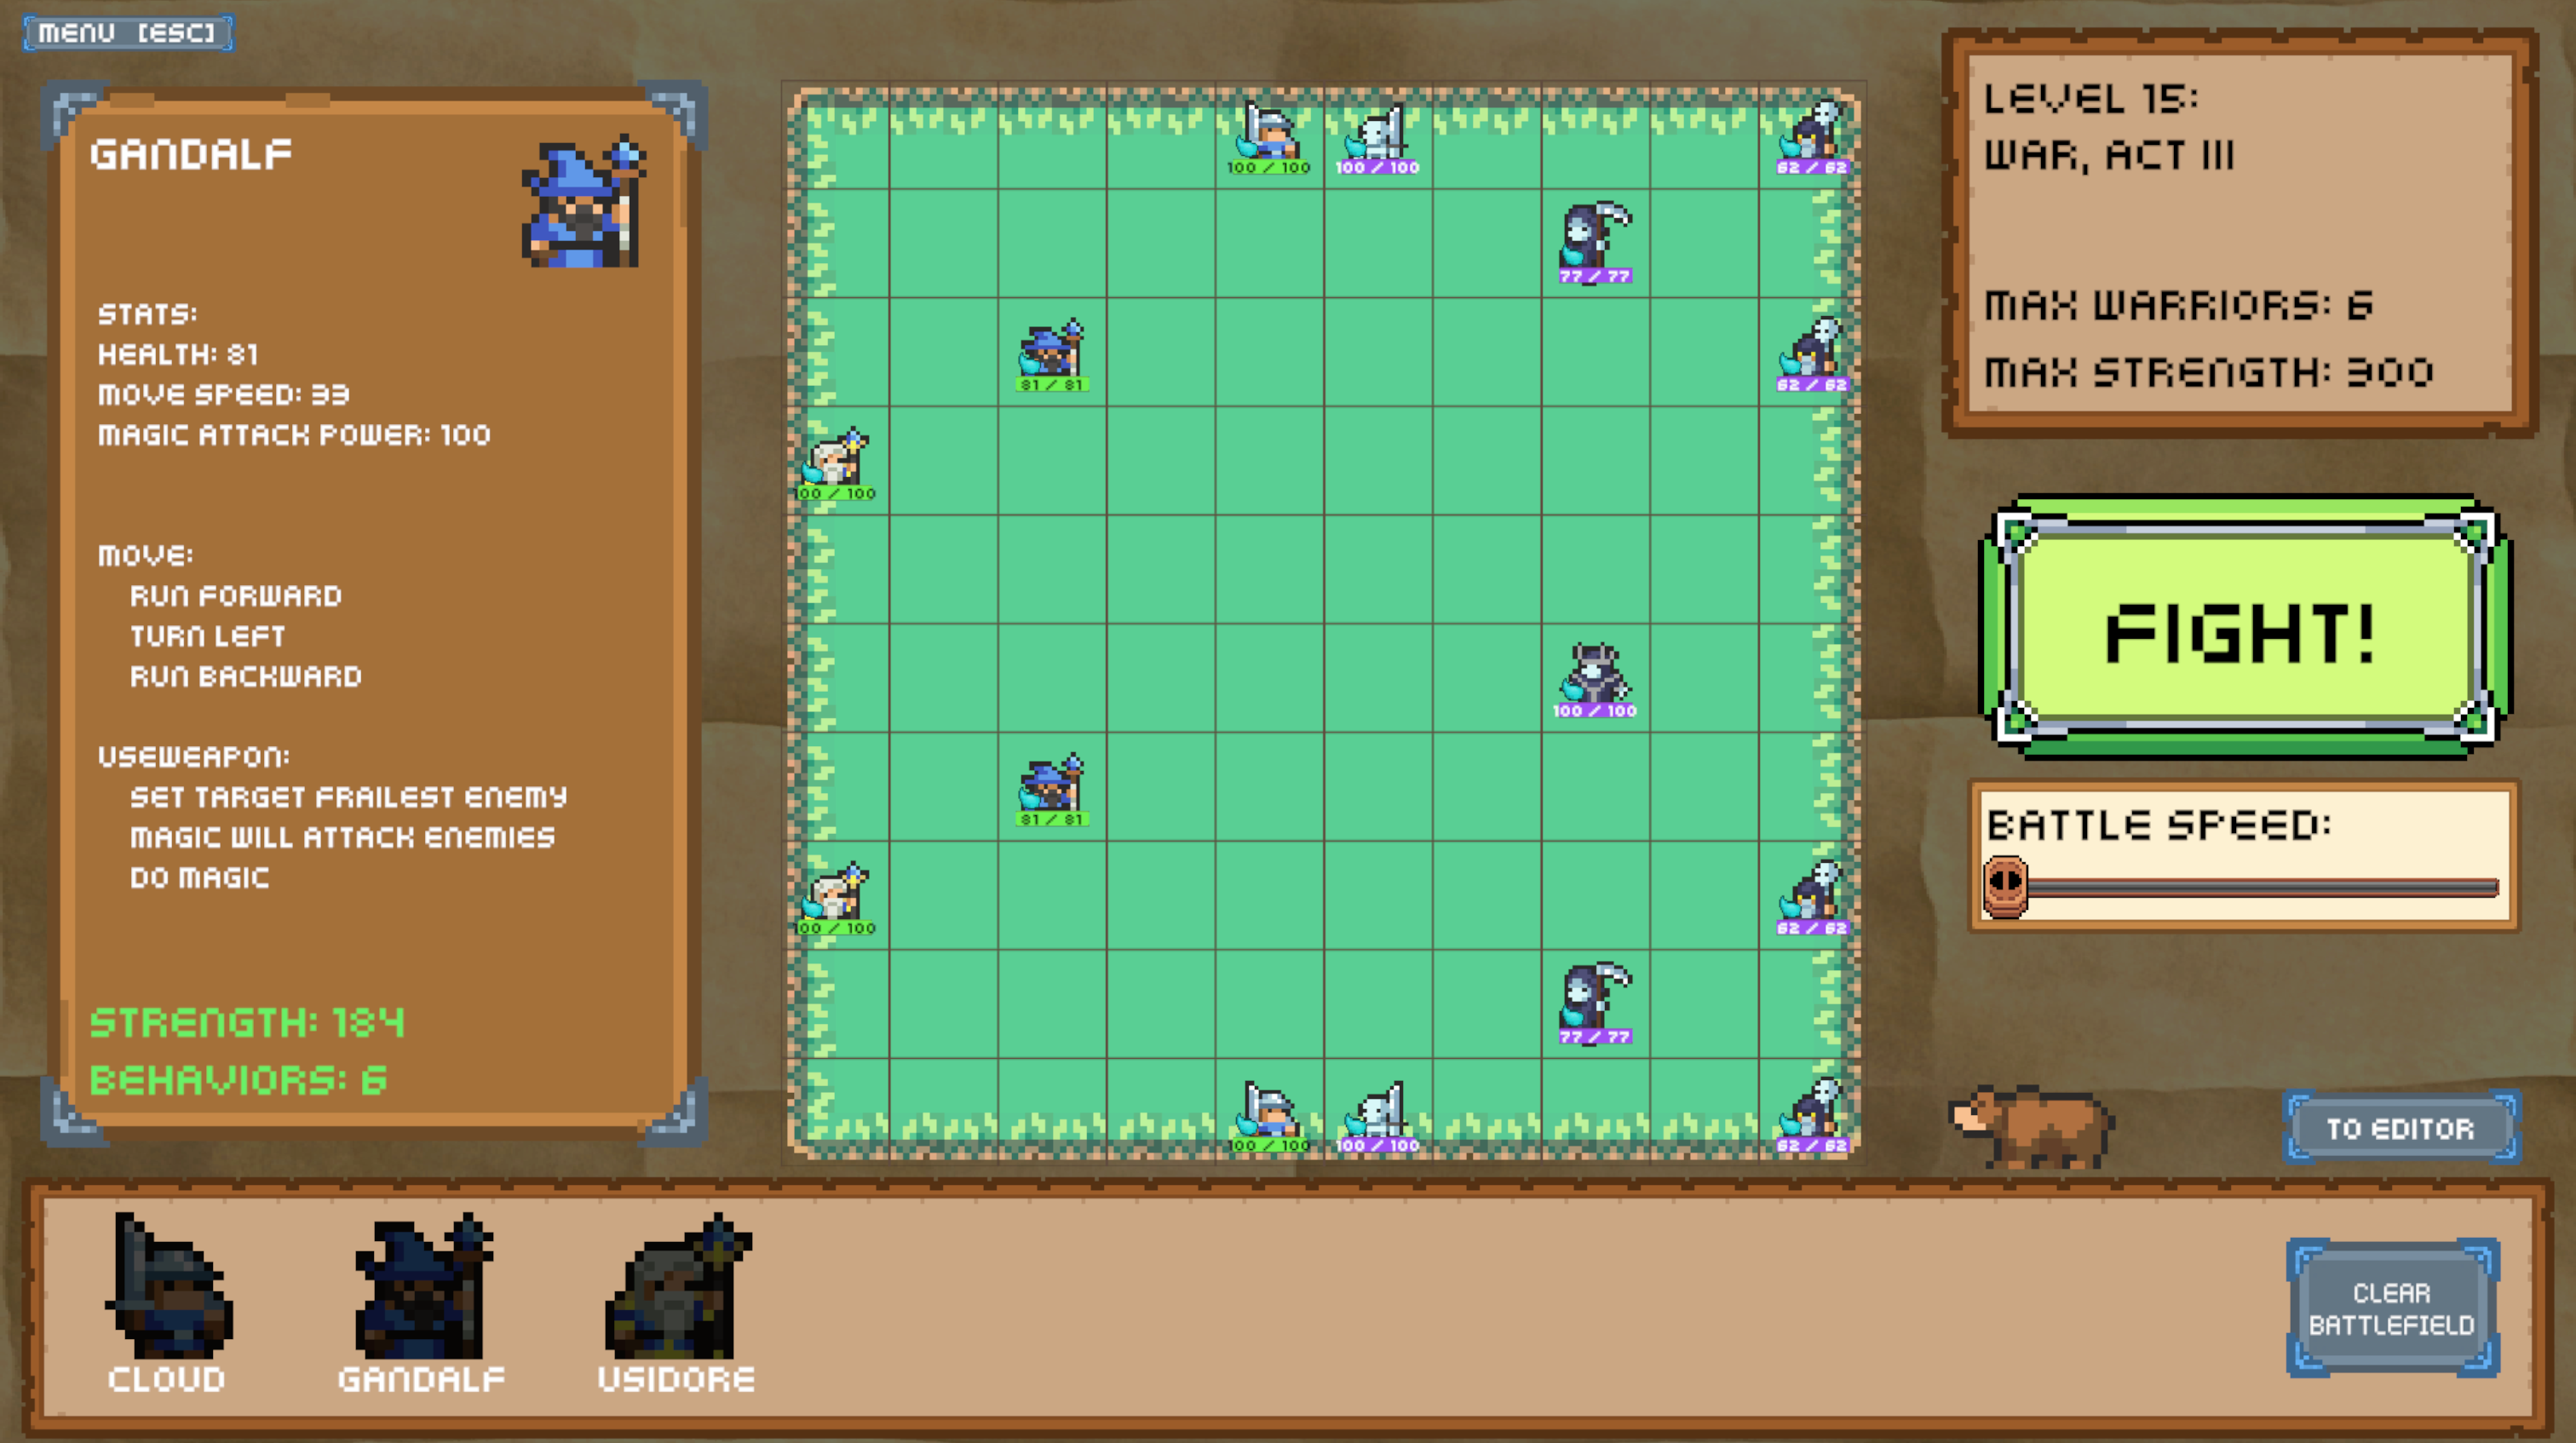
\includegraphics[width=\linewidth]{images/screenshots/level_setup.png}
    \caption{Warriors and enemies are placed on the battlefield in level fifteen.}
    \label{fig:level-screenshot}
\end{figure}

One critique of GBL within the classroom is that implementation can be resource intensive, requiring curriculum alteration, and may be less successful due to attitudinal factors \cite{drivers-barriers}. However, this same paper further describes how both gamification and GBL are highly useful tools if they are able to be implemented around the aforementioned barriers. To this point, a 2020 study on the benefits of using a game-based lecture (in comparison with a traditional lecture) showed an increase in attentiveness, collaboration, and excitement about learning the course material for both Urban Planning and Computer Science students \cite{game-on-gbl}. 

Gamifying computer science is not a new concept, but despite its proven effectiveness, Stephen Foster \cite{coding-game-design} identifies the lackluster success of coding games outside of an educational context. This is in large part due to the fact that most coding games are either unapproachable due to UI or installation issues, or that many never reach a stage beyond prototyping. For further development, Foster outlines three types of coding games: “coding in a game”, “coding as a game”, and “coding for a game”. \textit{Magicode} fits somewhere between the first two categories, which are defined by having an integrated coding interface, and having the gameplay itself be a form of coding, respectively. The final category has to do with programming game modifications, though that is unrelated to my project.

As found in a 2022 survey of gamification and GBL in K-12 classrooms over the last decade \cite{guan-gbl}, GBL is just as effective of a teaching methodology for younger students as it is for older students. Notably, this survey highlights that children are now more than ever in constant interaction with technology and video games, and providing students with an educational tool that offers a positive, cognitively-stimulating experience is critical to their learning how to use technology effectively. My project seeks to serve this purpose: by playing a game that is both fun and educational, students will learn fundamental computer science concepts and want to continue their learning both through the game and in the classroom.



\section{Methods}
This section explores the design and development process of \textit{Magicode} through its iterations, educational frameworks, and writing of a Game Design Document (GDD).


\subsection{Gameplay}
In \textit{Magicode}, the player takes on the role of a king who travels the land to defeat a looming threat of evil. Using the powers of drag-and-drop coding bestowed upon them by their non-player character (NPC) companion Garth, a talking bear, the player creates an army of knights and wizards to battle through increasingly difficult hordes of enemies, all the while learning the fundamentals of programming.

\begin{figure}
    \centering
    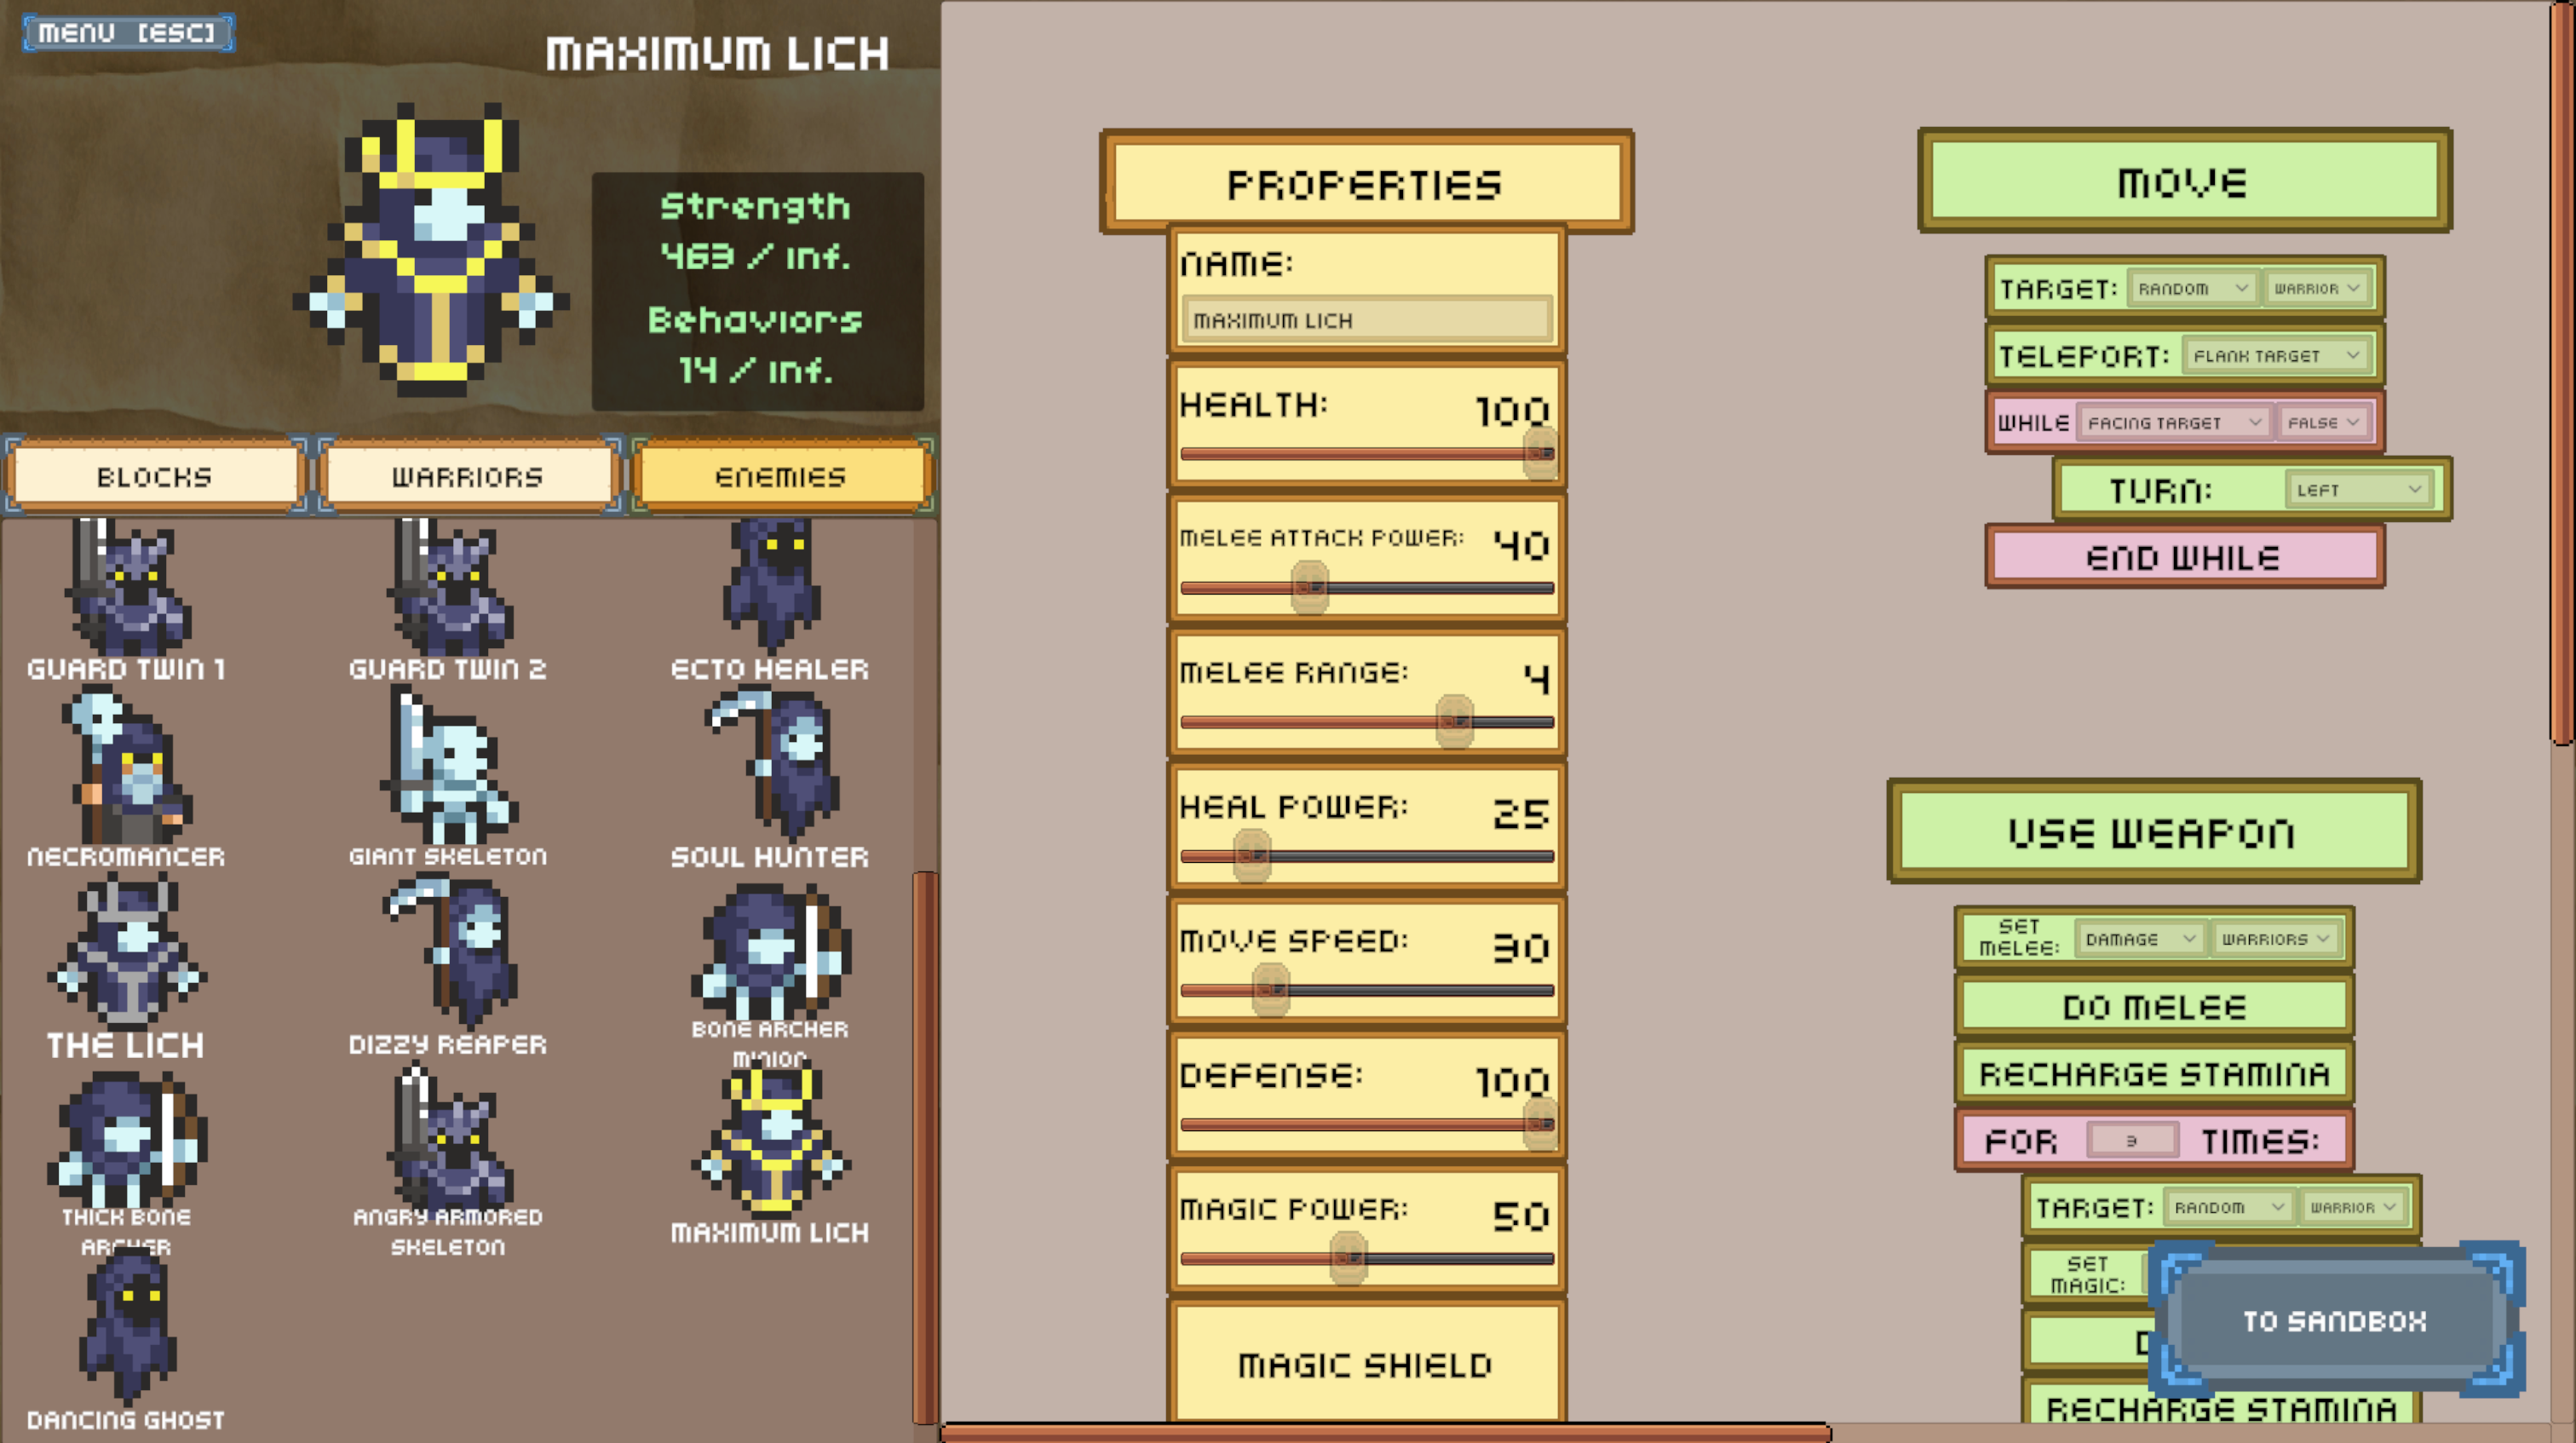
\includegraphics[width=\linewidth]{images/screenshots/lich_editor.png}
    \caption{The code editor with readable enemy code.}
    \label{fig:enemy-screenshot}
\end{figure}

Upon entering a new level, Garth presents the player with an interactive tutorial that walks them through the level’s new mechanics and enemy placements. Dialogue in the tutorial also develops the game’s story, describing the narrative scenario in which each level is set. From here, the player is given free reign to experiment with the drag-and-drop coding language in the Code Editor (Figure \ref{fig:code-editor-screenshot}) to design warriors to fight in battle. Once the player is satisfied with their designs, they transition to the Battlefield (Figure \ref{fig:level-screenshot}), where the actual battle will occur. All enemies that the player fights are programmed using the same in-game drag-and-drop language that the player uses (Figure \ref{fig:enemy-screenshot}). This allows players to learn how to read code as well as write it, and careful analysis of enemy code will provide players with examples of how they should solve each level if they feel stuck. Pressing the fight button initiates the battle, and the player watches as their warriors fight enemies automatically, following the behavior that they programmed. The battle will be successful only if key programming concepts are understood and correctly implemented. If the player does not succeed, they are prompted to continue editing and experimenting until they are able to progress. The flow diagram of each level’s gameplay can be seen in Figure \ref{fig:level-loop}.

\begin{figure}
    \centering
    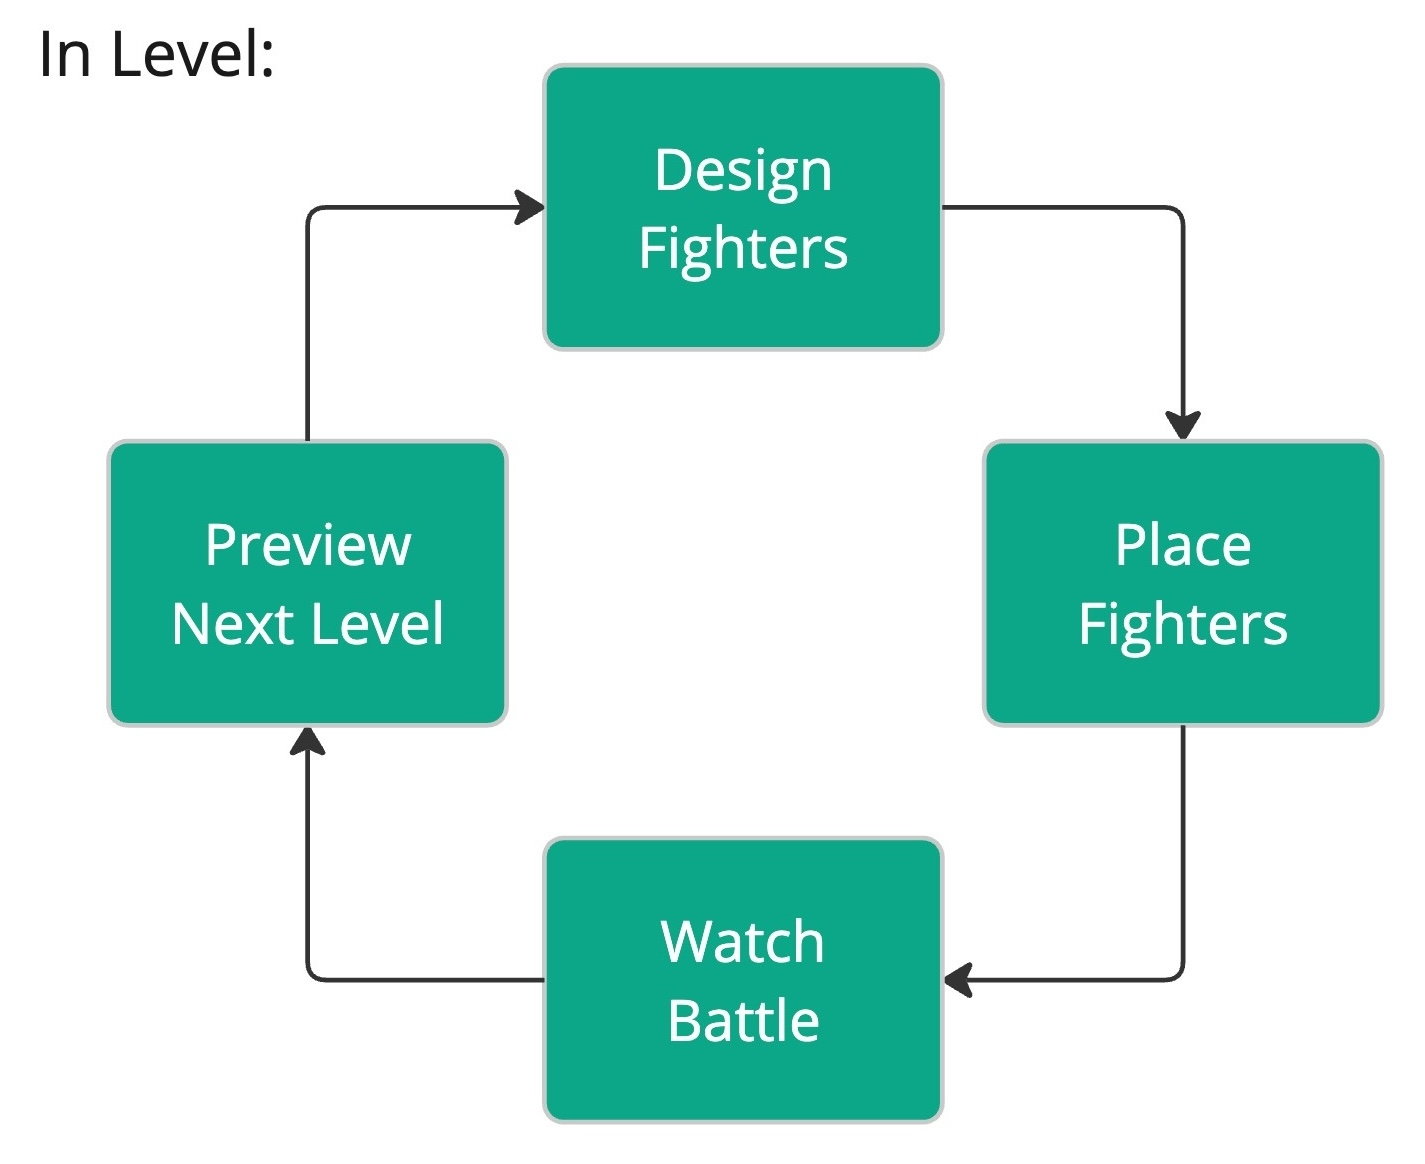
\includegraphics[width=.7\linewidth]{images/level-loop.jpeg}
    \caption{The level gameplay loop for \textit{Magicode}, diagramming player's moment-to-moment flow in each level.}
    \label{fig:level-loop}
\end{figure}

Progression through \textit{Magicode} sees the player learning a new concept, applying it effectively in a new level, and unlocking new levels through their success. The flow of this progression can be seen in Figure \ref{fig:metaprogression-loop}.

\begin{figure}
    \centering
    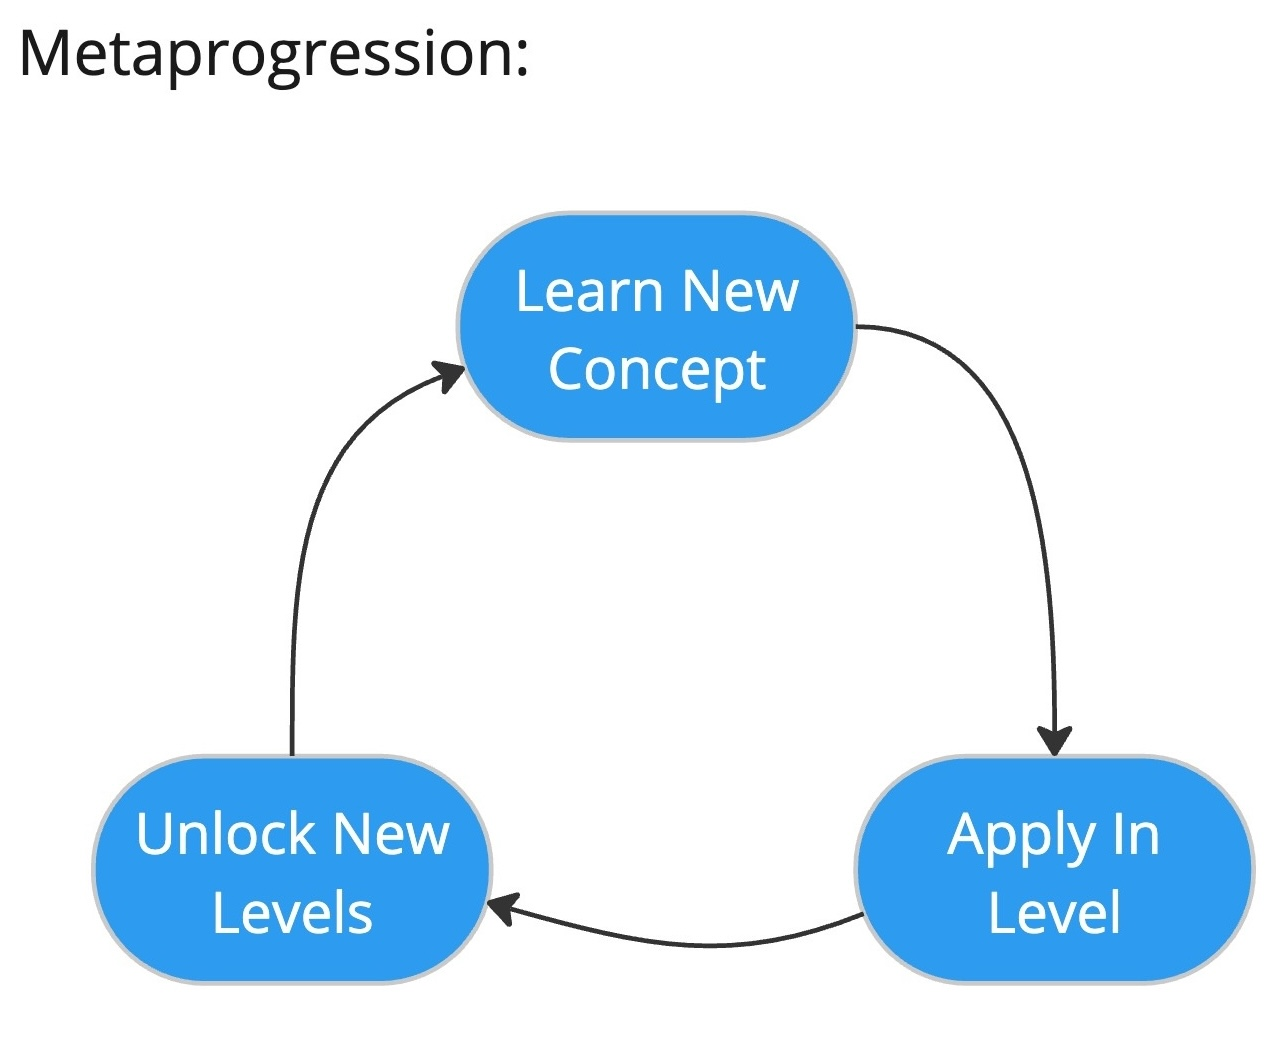
\includegraphics[width=.7\linewidth]{images/metaprogression-loop.jpeg}
    \caption{The metaprogression loop for \textit{Magicode}, diagramming what happens between levels.}
    \label{fig:metaprogression-loop}
\end{figure}

Outside of the structured levels is the Sandbox, a separate Code Editor and Battlefield without limits or predefined conditions required to complete a level. Instead, players can freely construct warriors using all possible code blocks without restrictions and, while they are not permitted to edit enemies, they are able to place an unlimited number of both their warriors and enemies onto the Battlefield. Figure \ref{fig:sandbox-battle-screenshot} shows a sandbox battle in progress, and Figure \ref{fig:sandbox-warrior-screenshot} shows a warrior designed for the sandbox.

\begin{figure}
    \centering
    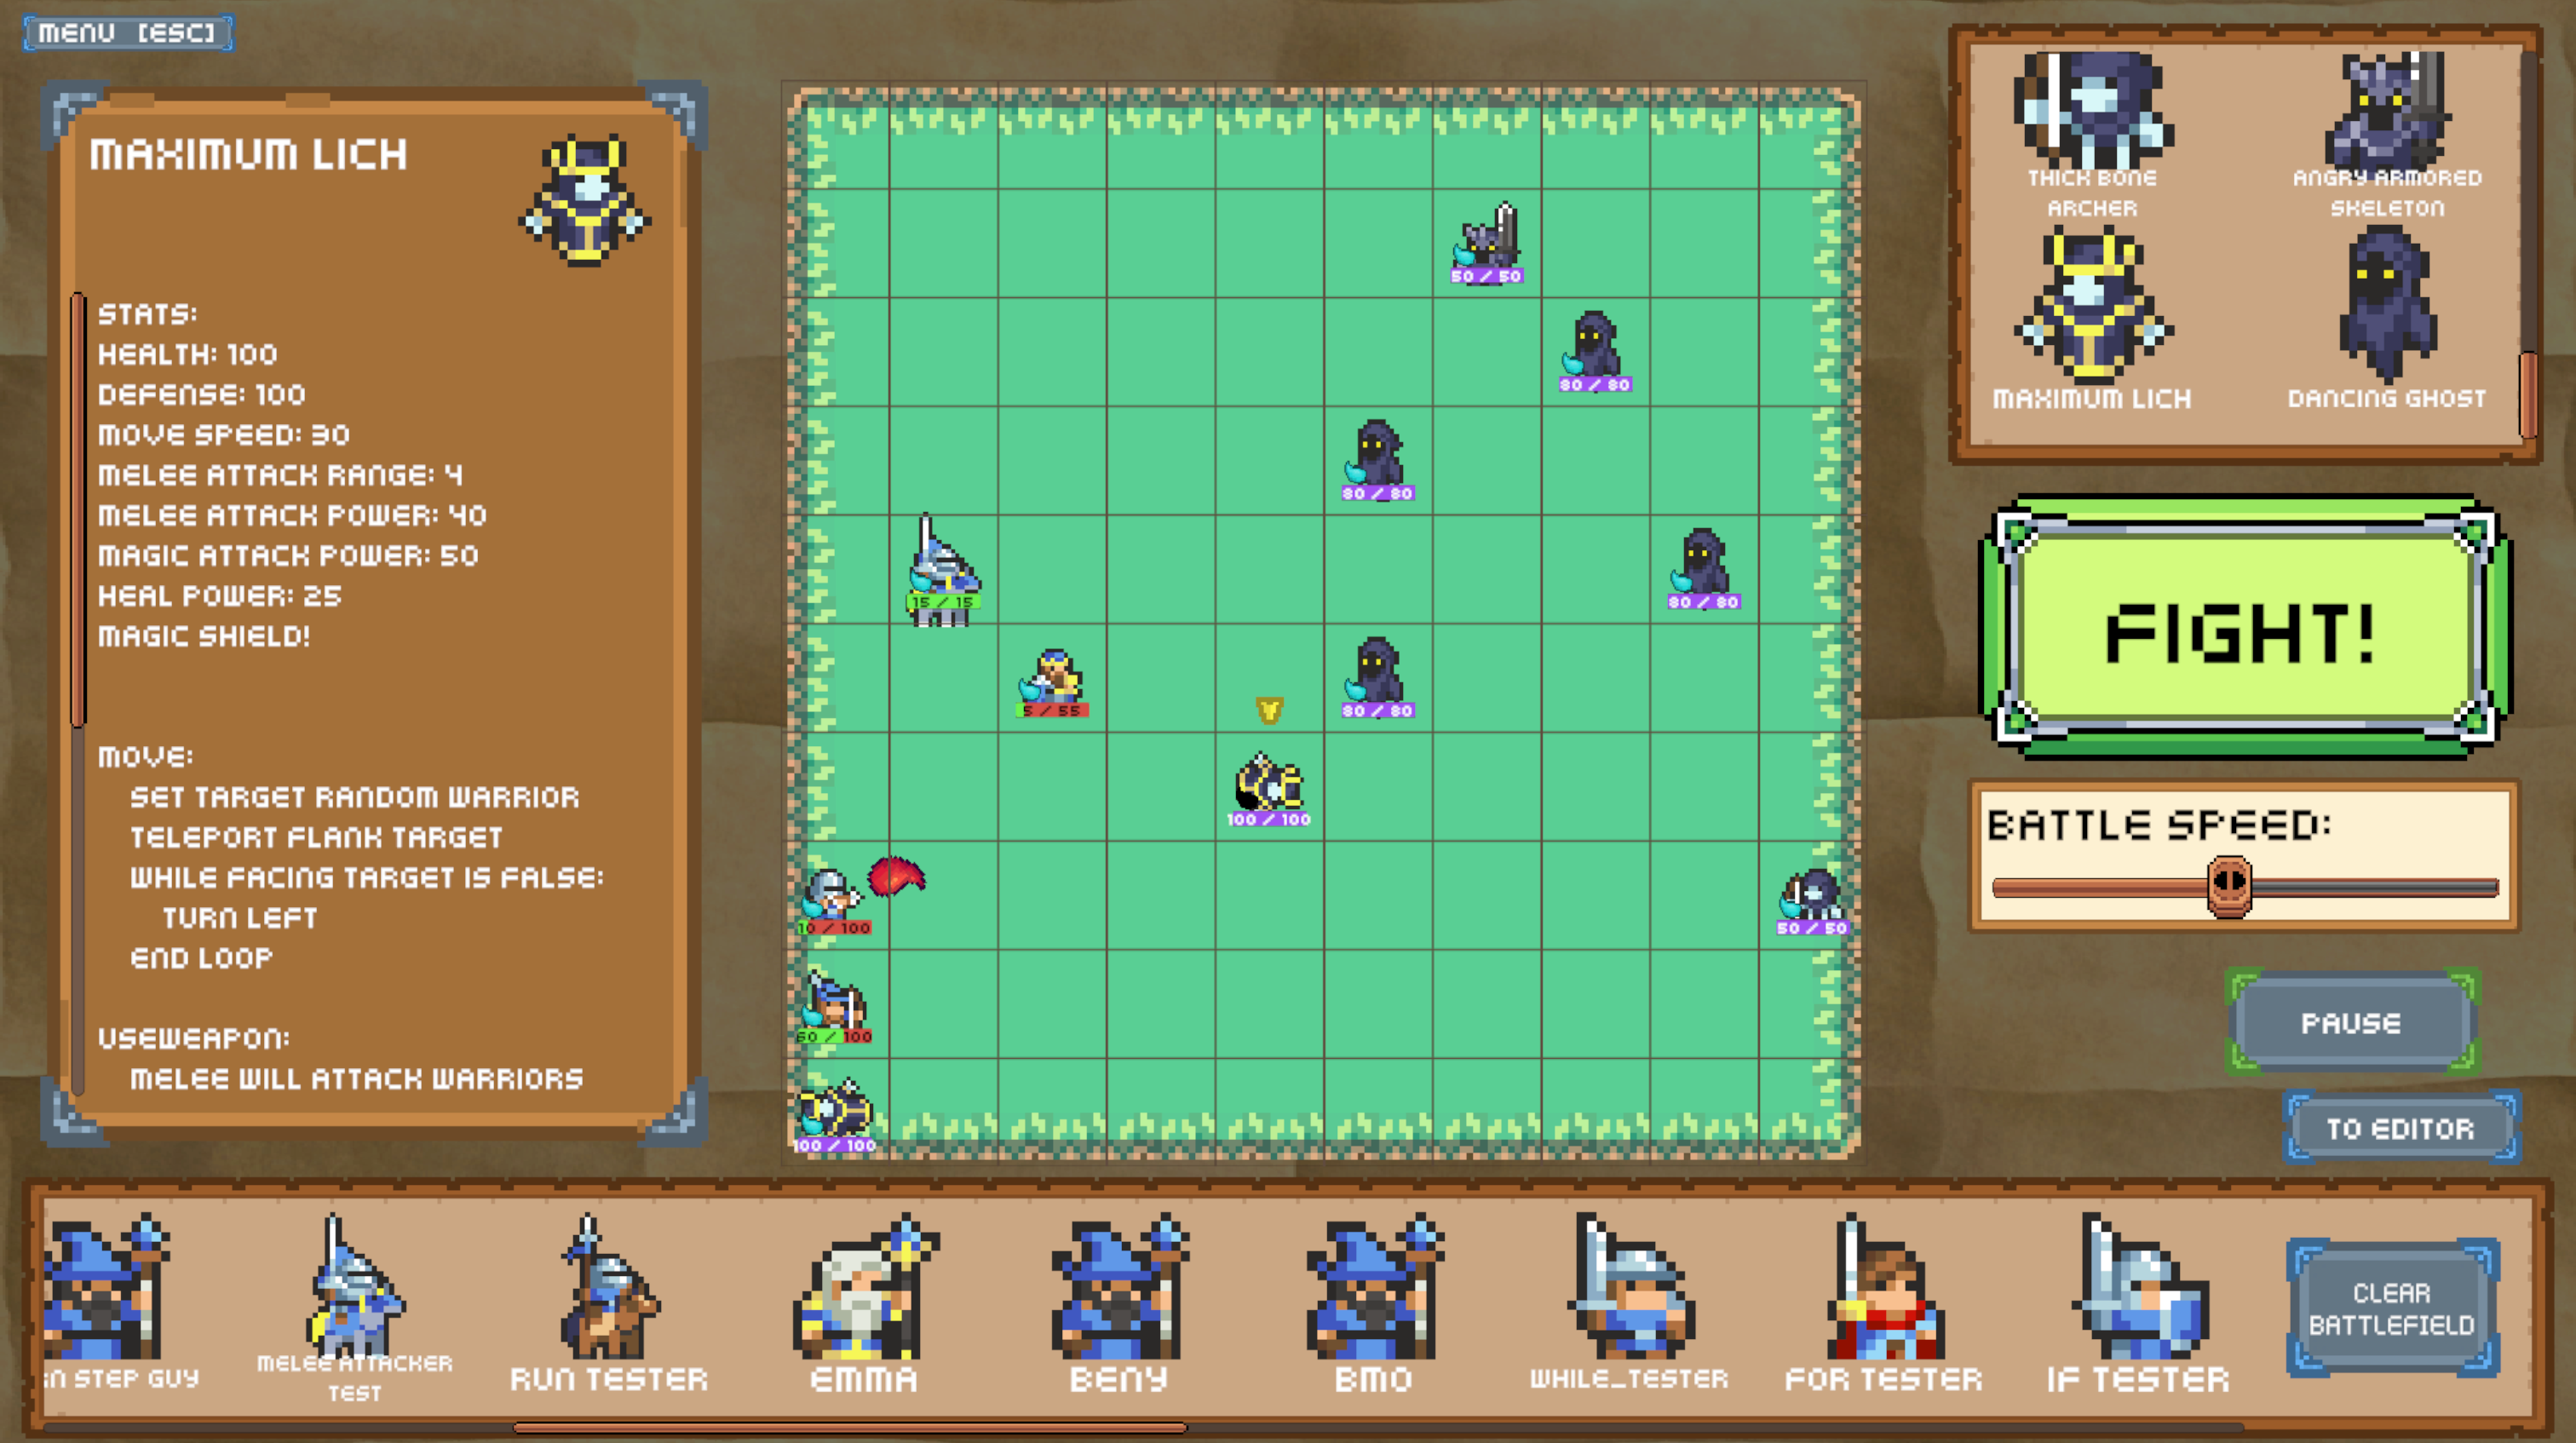
\includegraphics[width=\linewidth]{images/screenshots/sandbox_battle_3.png}
    \caption{A battle in progress in the sandbox.}
    \label{fig:sandbox-battle-screenshot}
\end{figure}



\subsection{Educational Design}
\textit{Magicode} implements BTEO at the core of its Game-Based Learning design. Each of its six steps are concretely implemented into the game’s level structure.

\begin{figure}
    \centering
    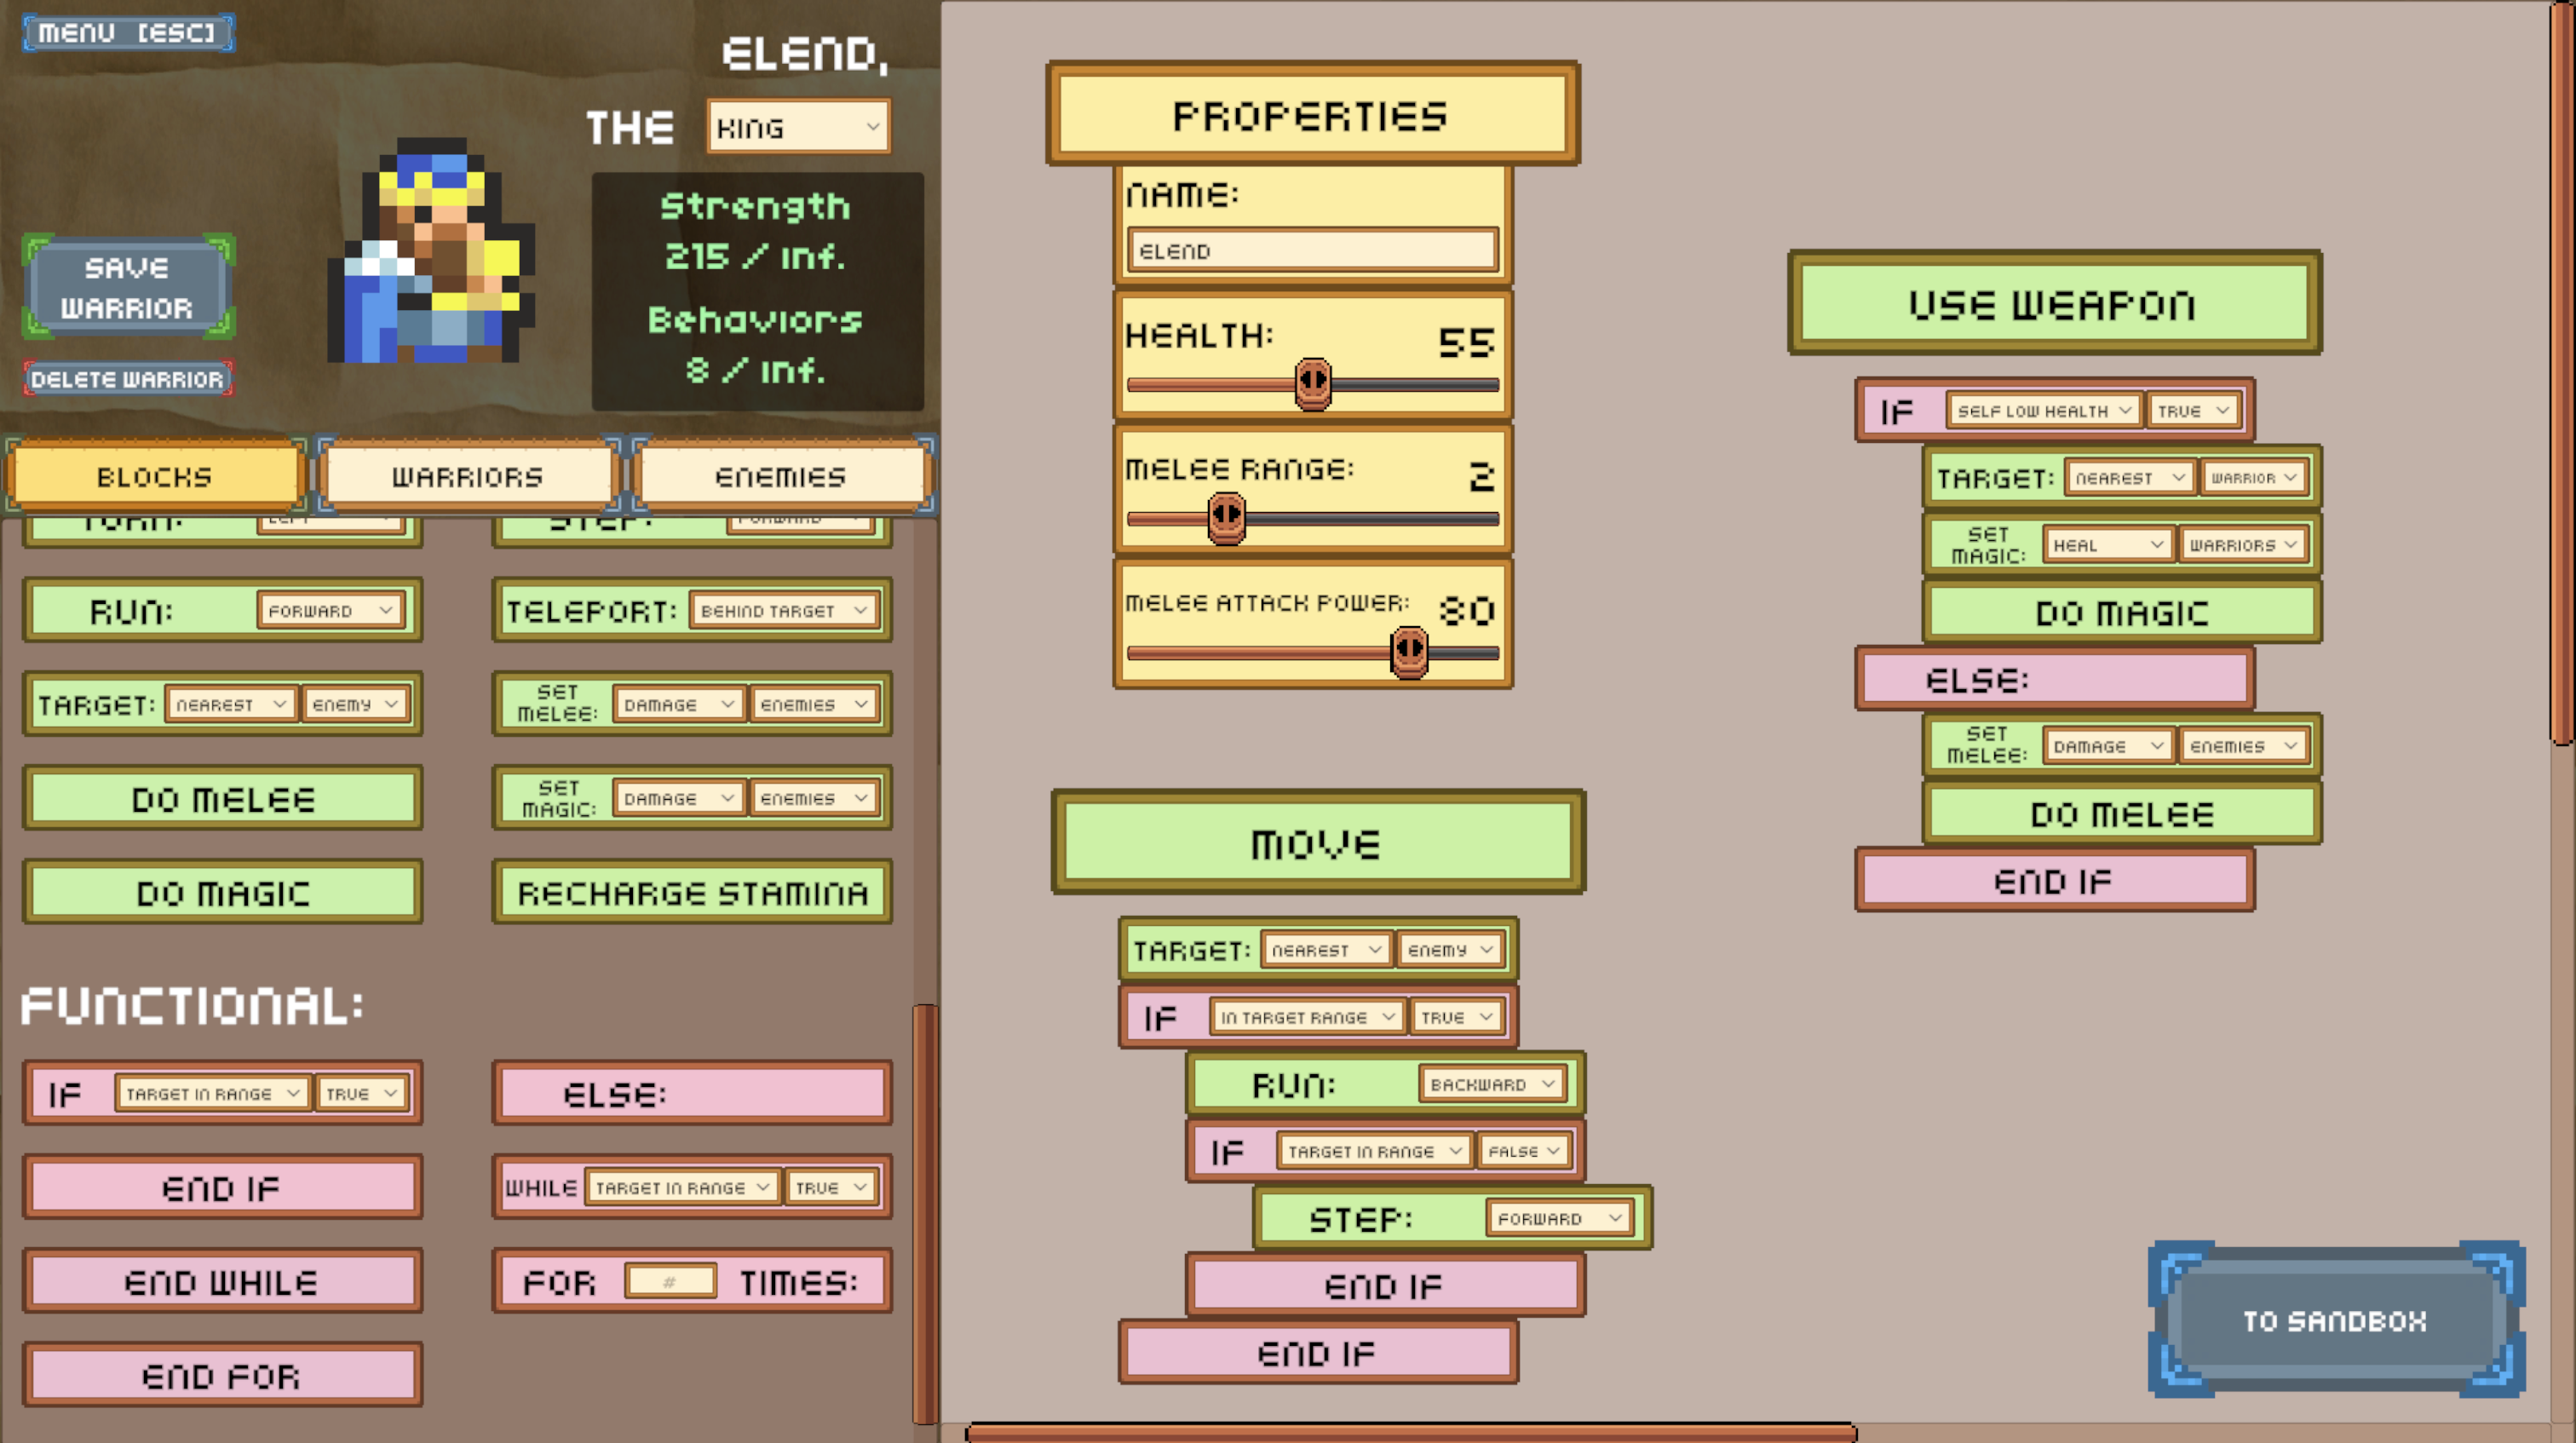
\includegraphics[width=\linewidth]{images/screenshots/elend_editor.png}
    \caption{The sandbox code editor featuring a much stronger warrior.}
    \label{fig:sandbox-warrior-screenshot}
\end{figure}

\textit{Knowledge}: Each level’s tutorial provides the player with new knowledge through new code blocks (Figure \ref{fig:tutorial-screenshot}). By using new blocks as described by the tutorial, players will show their baseline knowledge.


\textit{Comprehension}: For each level that introduces a new code block, all possible solutions require its usage. Comprehension can be shown by solving the level using the new mechanics, although players at this stage do not need a full understanding of how the new block connects with all other code blocks.

\textit{Application}: To take a step further, players are required to apply their knowledge and comprehension of existing mechanics to build their solutions for later levels by effectively using older code blocks.

\textit{Analysis}: Reading and understanding enemy code is critical to understanding how each level works. All levels require the ability to analyze code in some form, although later levels require a deeper level of analysis.

\textit{Synthesis}: Players will synthesize their knowledge through effective placement of warriors on the battlefield. This requires an understanding of the relationships between the objects that they have analyzed in order to succeed in each level.

\textit{Evaluation}: While external evaluation comes in the form of level success or failure and completion of the game, internal evaluation is the ultimate goal of \textit{Magicode}, where players should be able to evaluate the outcome of a battle before ever clicking the button. This should be attained by the end of the game through a reasonable level of difficulty and enough levels to allow players time to learn mechanics and concepts thoroughly.

\begin{figure}
    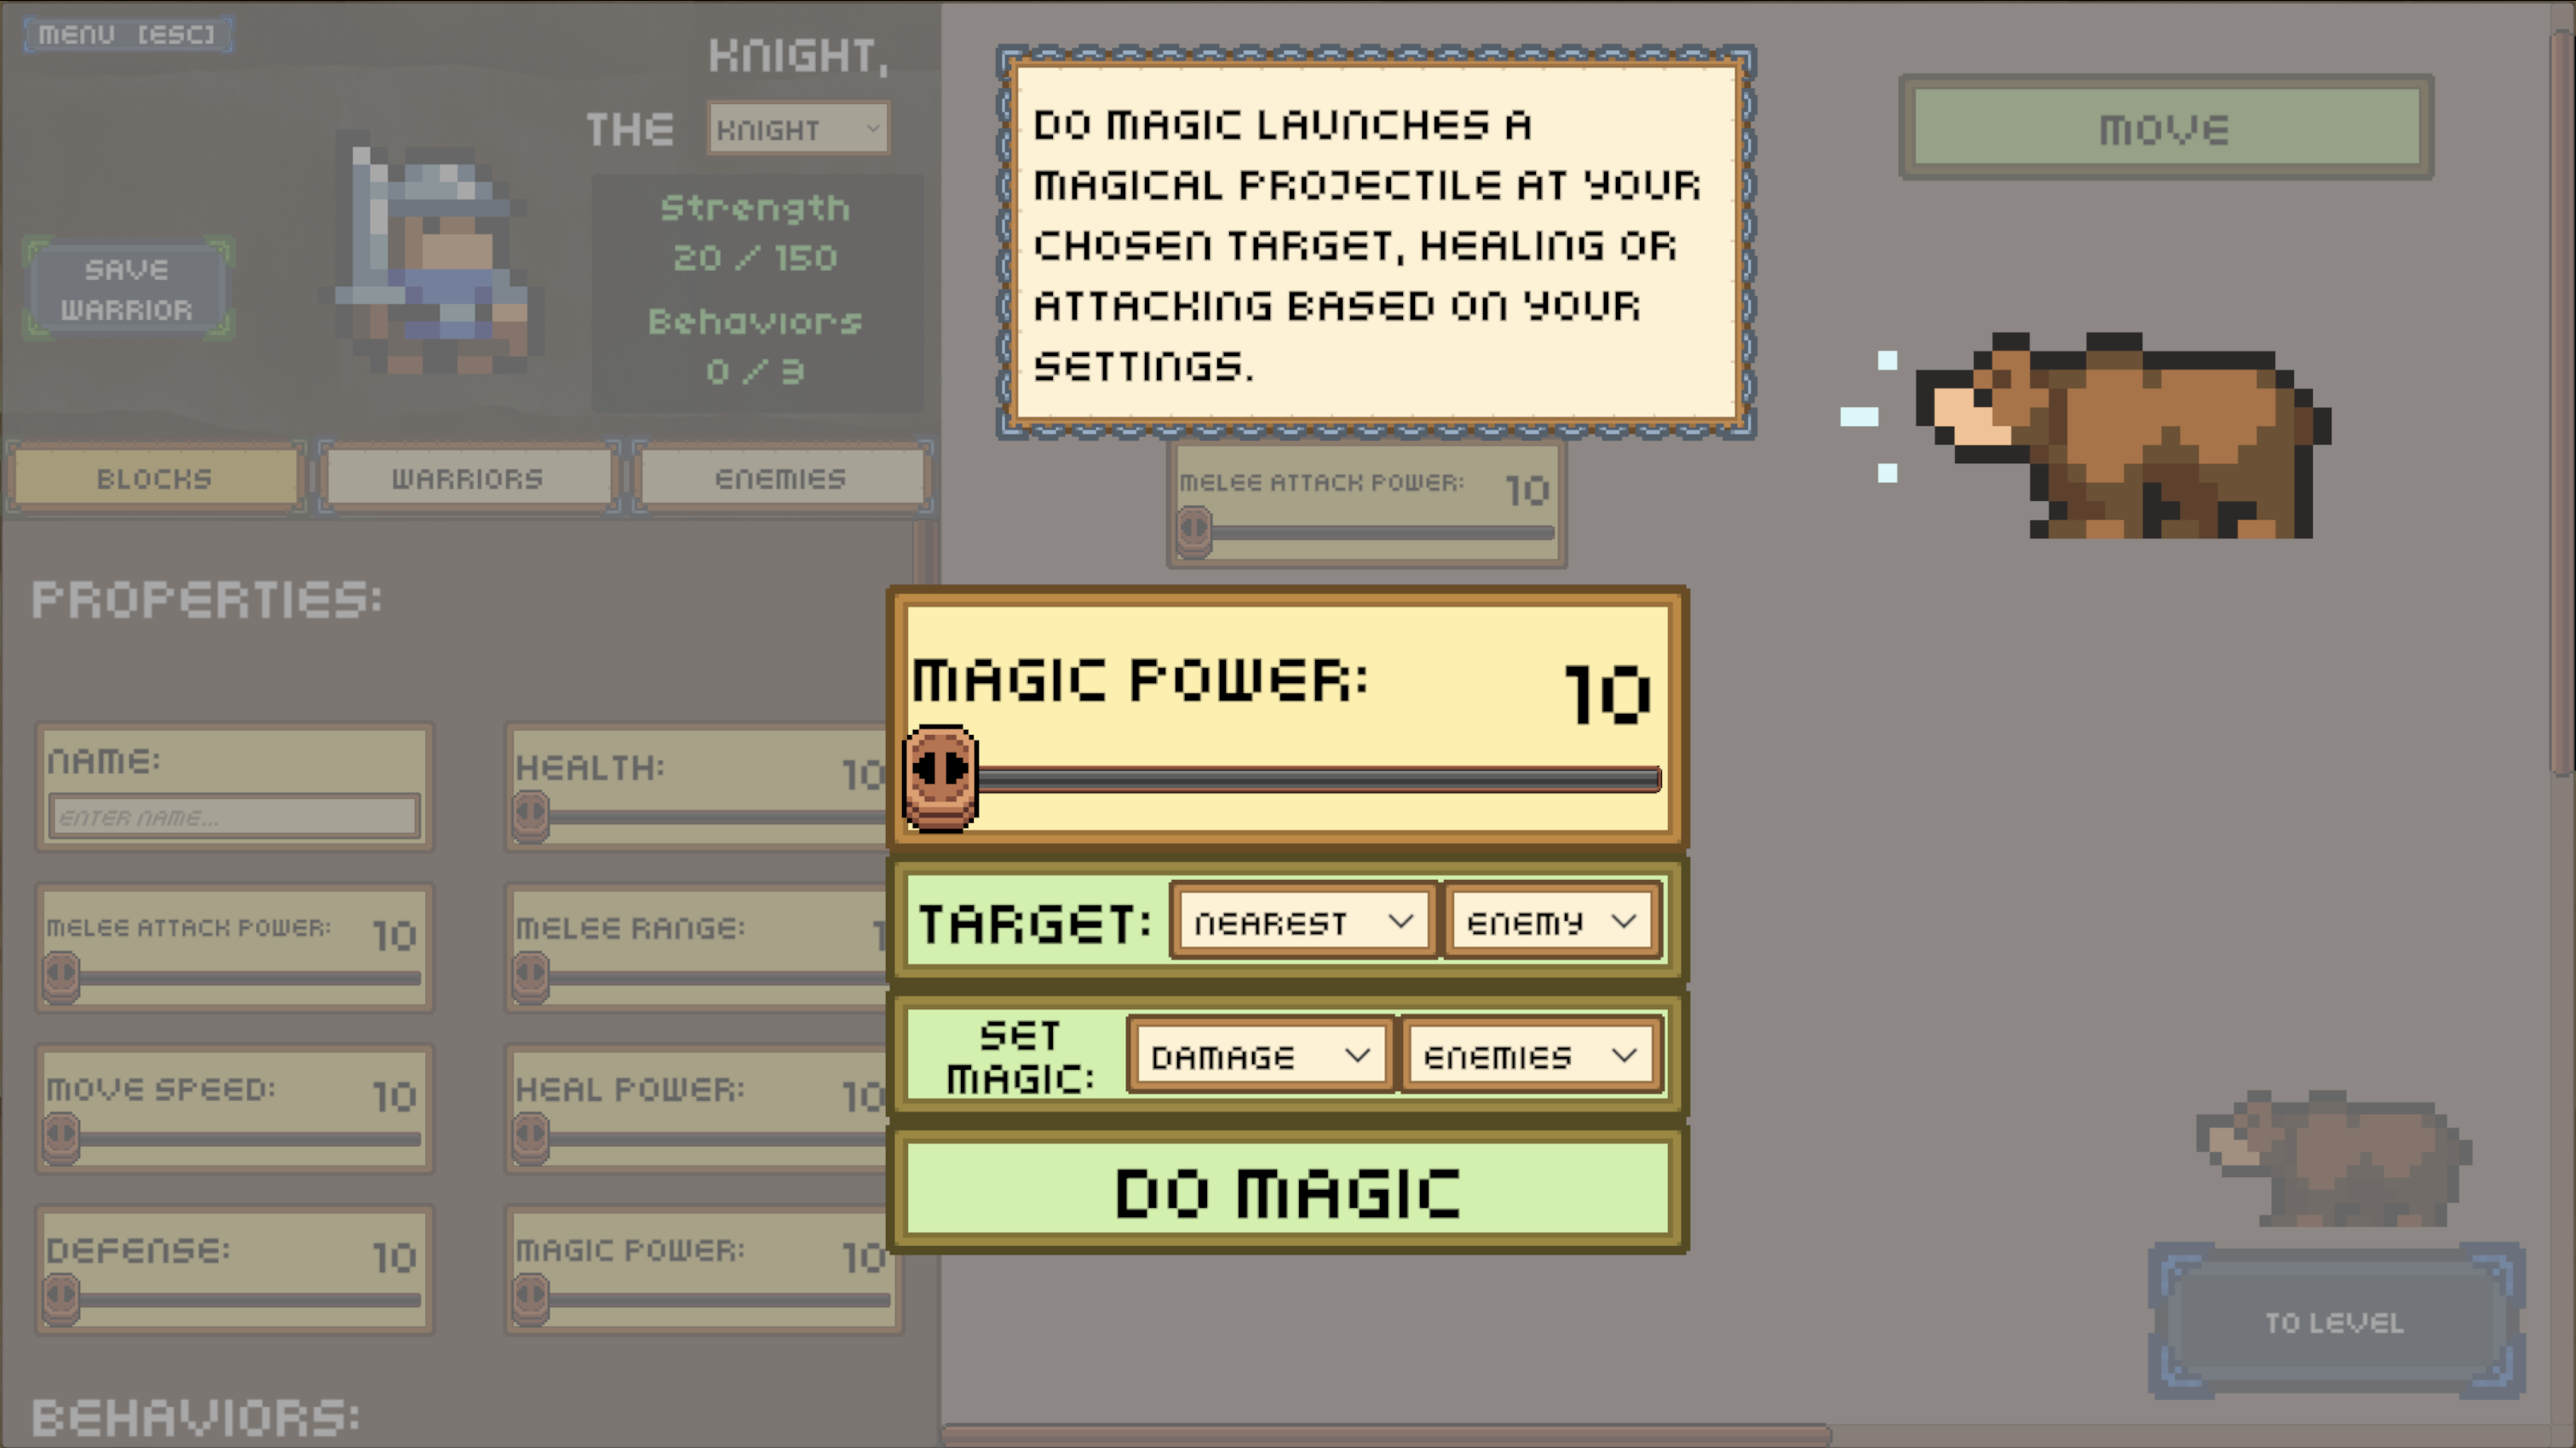
\includegraphics[width=\linewidth]{images/screenshots/tutorial.png}
    \caption{A tutorial in progress, showcasing new blocks available in the level.}
    \label{fig:tutorial-screenshot}
\end{figure}

The game’s difficulty is generally low, which is an intentional choice to prioritize learning and experimentation instead of punishing players for failure. This encourages players to continue when they do not succeed, requiring very little outside motivation. Interactive tutorials at the start of each level hint the player toward possible solutions and ensure that players do not miss any core mechanics.

Levels are sequenced such that very few code blocks and enemies are introduced initially, and only one or two new mechanics are included in each level. The first five levels introduce players to the core mechanics of properties and simple behaviors, with the next five adding one additional function header and more complex behaviors. Once players feel comfortable with the basics of function sequencing (through behaviors) and variables (through properties), levels eleven through fifteen introduce conditionals and branching, adding a layer of complexity. Lastly, levels sixteen through twenty introduce looping, giving players an additional dimension of their code to consider. Though the volume of possible solutions for each level increases with the addition of new code blocks, enemies are designed to prevent players from progressing without using the new code blocks in their solutions.

\subsection{Iterative Prototyping}
Early stages of each iteration of development involved prototyping by developing the simplest implementations possible of each gameplay mechanic to communicate the idea of what a fully functional game may look like. User testing with prototypes, especially early in development, is a necessary step to ensure that the developer’s internal ideas are effectively being externalized through gameplay \cite{prototyping}. When developing a game, one can very quickly discover that planned mechanics are not as fun or effective as intended, thus it is important to leave room in the prototyping process to experiment and discover alternative design approaches. This phase of designing \textit{Magicode} involved creating new coding blocks, experimenting with a wide range of level designs, and testing different ways to introduce the player to new mechanics and educational content.

Throughout the development process, I received feedback in two forms: in-class, through presentations and peer feedback, and outside of the classroom, through informal user testing. Core mechanics of \textit{Magicode} were scrapped and replaced, especially early in development, due to in-class feedback. Though my initial design was for a game about Object-Oriented Programming, early feedback revealed that the concept was beyond the scope of this project, and thus major structures of the game were reconsidered. The presentation process also allowed for greater clarification of my game’s design and its core mechanics, as the repetition of explaining and re-explaining led to a clearer vision of the game with more focused mechanics.

The final version of the game was evaluated through a formalized user testing process that is explored in the following sections, but informal user testing was critical to implementing changes before that point. For example, early playtesters noted a lack of clarity in what each code block does, leading to the creation of the tooltip system, where hovering the mouse over a code block reveals a brief description of how it can be used. I discovered that players who were less familiar with common video game terms (e.g. “health” and “attack” as character stats) struggled considerably, as they are never explicitly explained. Instead of adjusting the game’s language to explore this, I opted to shift the game’s target audience, and continue designing for players who would be more familiar with video games but less familiar with code. This was done to ensure that players did not feel overwhelmed by needing to learn too much at once, and that the educational content could be the only thing that the player needed to focus on.

As these changes were implemented, I updated the GDD to reflect new design choices. The motivation between alternating between building prototypes and writing the GDD is to allow these two phases of development to implement each other directly.


\subsection{Game Design Document}
The purpose of a Game Design Document is not only to keep track of my own progress, but also to provide a clear and concise way for others to learn about \textit{Magicode} and its development process. The GDD is broken into the following sections, adapted from Jukka Haltsonen’s \cite{gdd-guide} GDD outline:

\textit{1. High Concept:} This section includes a short description of the game’s purpose, who the game is designed for, and the objectives of those players. It also outlines what will be detailed in later sections, as well as a plan for the game’s release.

\textit{2. Gameplay:} The following section breaks down the key gameplay loops, exploring the design of each aspect of the game the player will interact with. Player actions and interactions with core systems are described in detail. This is necessary to refine the game’s structure and ensure that nothing is being unnecessarily overcomplicated by the developer.

\textit{3. Character/World Design:} Here I describe the characters and world of my game, explaining their backstories and motivations alongside samples of art and descriptions of musical tone. Due to time and budget constraints, the art and music of \textit{Magicode} are sourced from preexisting, royalty-free sources.

\textit{4. Educational Design:} The next section explores how \textit{Magicode} is designed with the Game-Based Learning framework. Here, the game’s learning objectives are stated alongside a description of their implementation through the structure of Bloom’s Taxonomy \cite{bloom-taxonomy}.

\textit{5. Technical Design:} My GDD concludes with an explanation of the backend algorithms and system controllers that make the game run.

\textit{Appendices:} Additional appendices include full documentation for \textit{Magicode}’s drag-and-drop programming language, individual level design details, and instructions for extending the game through new levels and code blocks.

While Haltsonen notes that each of these sections could be discrete documents in and of themselves, none are sufficient to serve as a complete design document without the others. Writing this document is a task admittedly large in scope, which highlights the value of an iterative design process. Alternating between prototyping features and writing documentation allows each step in development to influence the other. Inspired by the Short Game Design Document for Education (SGDDEdu) developed by researchers at Universidade Federal do Rio Grande do Norte Natal in Brazil \cite{gdd-ed-game}, the first step of my GDD development process was creating an outline with a strong description of the game’s high concept and learning goals. Once these foundations were solidified, I continued developing the living GDD with the addition of new gameplay mechanics. The document underwent many changes throughout the development process, and the final result is the product of an iterative design process shaped by feedback received and testing at all steps along the way.



\section{Evaluation Metrics}

Evaluation of \textit{Magicode}’s completion and success is measured with the following Project Goals (PGs):

\begin{itemize}[leftmargin=.5in]
    \item[\textbf{PG1:}] A fully playable game with a substantial amount of levels, as well as a sandbox level in which the player can freely experiment with the game’s systems.
    \item[\textbf{PG2:}] A completed Game Design Document.
    \item[\textbf{PG3:}] Full implementation of audio and visual effects.
    \item[\textbf{PG4:}] Players find \textit{Magicode} fun, yet reasonably challenging.
    \item[\textbf{PG5:}] Effective tutorials guide the player through the game’s educational content.
    \item[\textbf{PG6:}] Players show noticeable improvement in their foundational programming skills.
\end{itemize}

PG1, PG2, and PG3 are reasonably straightforward, necessary steps towards having a completed project. To measure PG4, PG5, and PG6, a group of twelve playtesters were given the same programming knowledge quiz both before and after playing the game. Quiz questions were selected from AP Computer Science Principles practice exams \cite{ap-practice-exam}, \cite{ap-practice-website} to test how well players understood the concepts of variable assignment, conditionals, branching, and looping. One sample question can be seen in Figure \ref{fig:question-9}. After completing the game, players filled out a survey to give qualitative feedback on a 7-point Likert scale, with prompts including:

\begin{itemize}
    \item “I enjoyed playing the game.”
    \item “I learned programming concepts that I was previously unfamiliar with.”
    \item “I felt like I could apply the programming concepts I learned to answer quiz questions more accurately.”
    \item “I found the tutorials helpful in teaching me new concepts.”
    \item “I feel like I could learn to code if I dedicated the time to it.”
\end{itemize}

Use of a 7-point scale over the traditional 5-point scale, a higher volume of narrow prompts, and additional free-response feedback all allowed for greater nuance in player response \cite{likert-explored}. This feedback is considered alongside the change in quiz scores recorded before and after playing \textit{Magicode} in an analysis of the game’s educational content through Bloom’s Taxonomy of Educational Objectives \cite{bloom-taxonomy}. Due to how introductory programming concepts naturally build on top of one another \cite{teaching-oop}, it follows that the hierarchical and cumulative nature of Bloom’s Taxonomy is an invaluable tool for designing and analyzing teaching structures for foundational concepts. This analysis will pertain to the following learning objectives for players (LOs):

\begin{itemize}[leftmargin=.5in]
    \item[\textbf{LO1:}] Gain familiarity with foundational programming concepts.
    \item[\textbf{LO2:}] Build confidence in programming skill and feel less intimidated by the idea of learning how to code.
\end{itemize}

Given that \textit{Magicode} can be played from beginning to end in a matter of hours, there is not enough time nor complexity to comprehensively teach players all there is to know about programming fundamentals. Rather, Learning Objectives seek to help players build a foundation and increase their confidence with programming concepts, providing them with transferable skills that can be used to further their Computer Science education. Success of these objectives will be measured through PG6.


\section{Results and Discussion}

This section examines to what extent each Project Goal was achieved. Additionally, a summary of the data collected is analyzed through BTEO.

\subsection{PG1: Completed Game}
Magicode consists of twenty fully constructed and balanced levels, as well as a sandbox level without restrictions. The full, playable game is available for download in the same \href{https://github.com/slevy14/Comps-Game}{GitHub repository} as this paper, as well as on \href{https://leafguy.itch.io/magicode}{Itch.io}.

\subsection{PG2: Completed GDD}
The completed Game Design Document includes all design details with justification, educational theories and their implementations, and both backend and in-game language documentation. To read the GDD, find the full document in the same \href{https://github.com/slevy14/Comps-Game}{GitHub repository} as this paper.

\subsection{PG3: Audio and Visuals}
All scenes have unique background music, and all actions have attached sound effects. These include drag-and-drop sounds, battle effects, and UI sounds for buttons and scene transitions. Each warrior and UI element uses customized animations and graphics; there are no instances of default Unity visual assets within the project. All audio and visuals are used under a Creative Commons license for personal use.\footnote{All visuals are sourced from various creators: \href{https://lyaseek.itch.io/}{LYASeeK}, \href{https://megatiles.itch.io/}{MegaTiles}, \href{http://kenney.nl}{kenney.nl}, \href{https://marie-pepo.itch.io/mf-items}{Marie Pepo}, \href{https://canarigames.itch.io/canaripack-8bit-topdown}{Canari Games}, and \href{https://bdragon1727.itch.io/basic-pixel-health-bar-and-scroll-bar}{bdragon1727}. All audio sources can be found for free at \href{https://freesound.org/}{freesound.org}.}

\subsection{PG4: Challenge and Fun}
Playtesting sessions lasted just under two hours each, including the quiz and survey taken by each tester before and after playing the game. Within this timeframe, only three out of twelve players fully finished the game, completing the twentieth level. Eight out of twelve players reached level eleven, however, where there is a notable increase in difficulty with the introduction of conditionals. Based on the pace at which most players progressed through the game, it can be reasonably assumed that a full playthrough would take an average of three and a half hours to complete. Most players reached level eleven at the end of their playtest session, unfortunately not leaving enough time for players to complete subsequent levels.

\textit{Magicode} received an average rating of 6/7, or an 85\%, for general enjoyment of the game from playtesters. In general, players enjoyed the game's difficulty, noting that the progression from one level to the next felt natural, and that their skill level was being fairly tested and built upon. With the slow introduction of new blocks and mechanics in each level, players never felt overwhelmed with the amount of options at their disposal. Players appreciated how levels were designed to prevent strategies that avoided intended solutions, thus requiring them to experiment and find a solution that took advantage of newly introduced mechanics. With experimentation at its core, the game never punished players for making mistakes, instead simply offering the option to retry a level and quickly correct their errors. This, combined with the visual and mechanical customizability of each warrior, led players to feel that their gameplay experience was truly unique and tailored to them.

Critiques and feedback received from playtesters were mostly requests for quality-of-life features and noting technical bugs. Common requests were an additional glossary or mechanical reference, options to duplicate warriors or save incomplete warriors, and additional visual indicators to mark a warrior’s range. Most of these features were initially planned to be included, but were never implemented due to time constraints. The lack of these features did not seem to hinder the gameplay experience, though they likely would have improved the experience of playing \textit{Magicode} for all players. Future work would include the development of these quality-of-life changes.

\subsection{PG5: Tutorial Effectiveness}
\textit{Magicode}’s tutorials are presented to the player in the form of a talking bear that explains each level’s new mechanics through a series of text boxes and highlighted UI elements. Figure \ref{fig:tutorial-screenshot} shows an example of one such tutorial. 75\% of playtesters found these tutorials to be helpful in some way, with only two respondents feeling neutral, and one feeling that they did not help. Although, as mentioned previously, some players wished for additional examples and a glossary reference, general feedback indicated that the tutorials adequately explained each level’s content and motivated them to continue playing. One player identified that, in addition to the explicit tutorial at the start of a level, the design of each level implicitly required use of new mechanics to progress forwards, citing this aspect as a highly successful teaching strategy.

The talking bear was a highlight for many players, with multiple survey responses praising its cute design as a form of engagement. All players reported feeling confident that they understood what the game expected from them; however, in playtest sessions, many playtesters asked questions to me directly regarding concepts that were explicitly stated in the tutorial that they just encountered. For example asking “how do I save?” immediately following a tutorial where the bear highlights the save button and instructs the player to click on it in order to save. This identifies a disengagement that some players felt by needing to read large blocks of text to continue playing, which could be adjusted in a future version of the game through more interactive and responsive tutorials.

Despite some initial struggles from some players at the beginning of their playtest sessions, 83\% of players found the UI easy to interact with. Players often spent an extensive amount of time in the game’s first level – designed to use both of the only two behavior code blocks that the player has available – just experimenting with the drag-and-drop system, property blocks, and warrior placement. Once players felt comfortable with the UI systems, they moved very quickly through the next few levels, and further continuing through the rest of the game at a consistent pace, taking the time needed to learn from each new level’s tutorial.

\subsection{PG6: Progress Towards Learning Objectives}
The first learning objective is for players to gain familiarity with foundational programming concepts. Regarding the nine question multiple choice coding knowledge quiz taken by players\footnote{Anonymized raw survey and quiz data is \href{https://docs.google.com/spreadsheets/d/1F7b50xaFvfE2F1knakdCm4rHaRKITp1pA6s78goNYoM/edit?usp=sharing}{linked here}.}, the median quiz score increased from 6.5 out of 9 before playing the game to 7 out of 9 afterwards, equivalent to a 7.6\% increase in average quiz score. Given that the vast majority of players were not able to fully complete the game during their playtesting session, this is a significant increase in score from playing just the simpler first half of the game. As an educational game, \textit{Magicode} is meant to give players an introduction to foundational concepts they can transfer to other coding languages. This increase in score points to \textit{Magicode}’s success as an educational tool. Qualitatively, all players who did not have any prior coding experience before playing the game reported feeling like they learned something new, and that they would be able to apply their new knowledge to the quiz. Of the three players who fully completed all levels in \textit{Magicode}, one of them achieved a perfect score before and after playing the game, but the other two showed substantial improvement in both score and comprehension.

Figure \ref{quiz-score-graph} shows the change in correct responses to each quiz question before and after playing the game. Questions 6 and 7 addressed variable assignment and manipulation, which are two concepts that \textit{Magicode} does not teach. The intention of their inclusion was to see if players developed a natural sense of computational thinking that would allow them to solve these problems, though the drop in correct answers signifies that players did not gain this skill. Question 1, which required players to understand how a nested loop would affect the movement of a robot on a grid, also had a slight drop in correct answers. This is likely due to the looping levels being at the end of the game, which many players did not reach, and therefore they were not able to apply that specific skill to the quiz. The most significant increase in correct answers can be seen in question 9 (Figure \ref{fig:question-9}), where respondents were asked to identify which two algorithms would move a robot from one point to another. This question required knowledge of both conditionals and loops, so the increase in score implies a stronger understanding of those concepts being attained after playing \textit{Magicode}.

The second learning objective is for players to increase confidence in their programming skill and feel less intimidated by the idea of learning how to code. On average, players reported a 13\% increase in confidence from the start of the play session to the end, and an even higher 17\% increase in confidence from players with no prior coding experience, as seen in Figure \ref{confidence-graph}. Given the high failure rates of introductory Computer Sciences courses at the collegiate level \cite{failure-rates}, this confidence boost,  alongside their foundational basis, could bolster players’ persistence through difficult introductory programming classes.


\begin{figure}
    \centering
    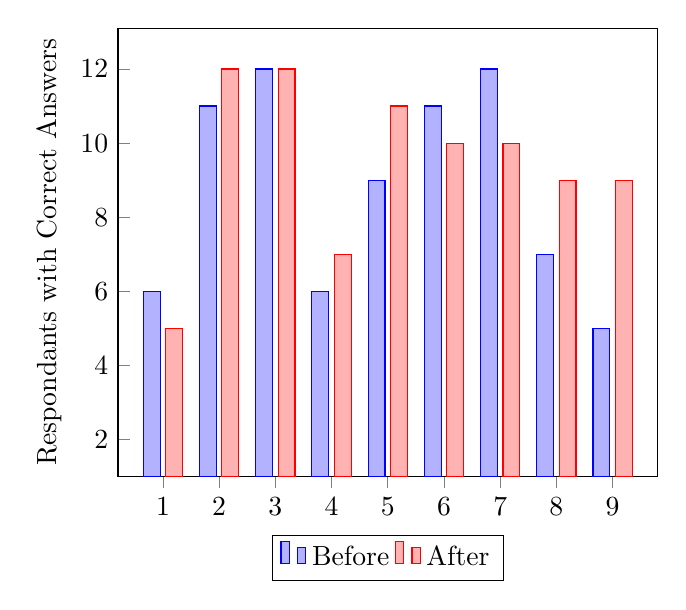
\begin{tikzpicture}
        \begin{axis}[
        	xtick = data,
                ylabel=Respondants with Correct Answers,
                legend style={at={(0.5,-0.13)},
                anchor=north,legend columns=-1},
                ybar,bar width=0.3,xtick pos=lower,ytick pos=left,
                ymin=1,
        ]
        \addplot 
        	coordinates {(1,6)(2,11)(3,12)(4,6)(5,9)(6,11)(7,12)   (8,7)(9,5)};
        \addplot 
        	coordinates {(1,5)(2,12)(3,12)(4,7)(5,11)(6,10)(7,10)   (8,9)(9,9)};
        \legend{Before,After}
        \end{axis}
    \end{tikzpicture}
    \caption{Change in correct responses for each quiz question before and after playing \textit{Magicode}.}
    \label{quiz-score-graph}
\end{figure}

\begin{figure}
    \centering
    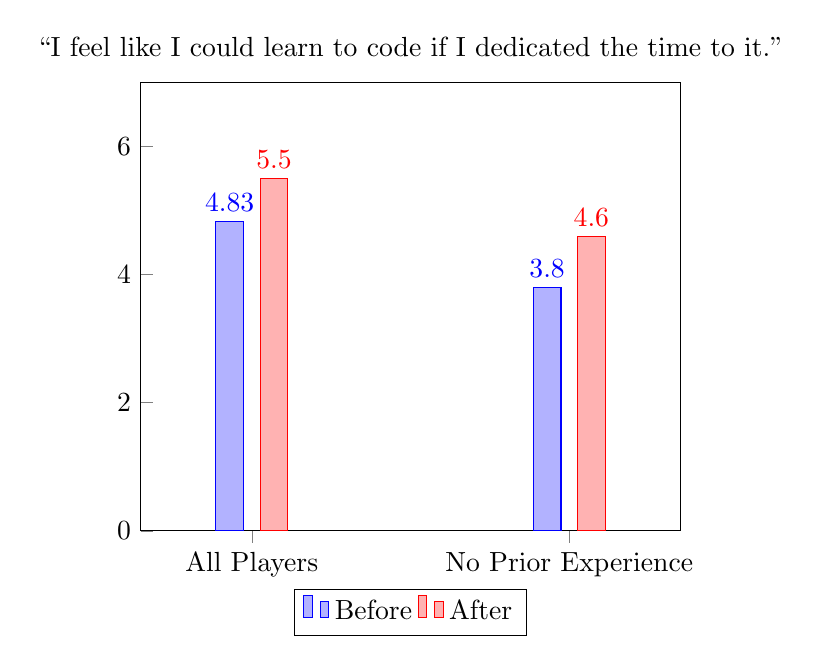
\begin{tikzpicture}
        \begin{axis}[
                title =  ``I feel like I could learn to code if I dedicated the time to it.'',
        	xtick = data,
                legend style={at={(0.5,-0.13)},
                anchor=north,legend columns=-1},
                ybar=6pt,xtick pos=lower,ytick pos=left,
                ymin=0, ymax=7,
                symbolic x coords = {All Players,No Prior Experience},
                nodes near coords,
                enlarge x limits=0.35,
        ]
        \addplot coordinates {(All Players,4.833) (No Prior Experience,3.8)};
        \addplot coordinates { (All Players,5.5) (No Prior Experience,4.6)};
        \legend{Before,After}
        \end{axis}
    \end{tikzpicture}
    \caption{Change player confidence before and after playing \textit{Magicode}.}
    \label{confidence-graph}
\end{figure}


\subsection{Analysis of Bloom's Taxonomy}
Finally, this data can be summarized through an analysis of Bloom’s Taxonomy of Educational objectives.

\textit{Knowledge:} Players found tutorials to be helpful in general, and quantitative data shows that they built a foundational knowledge basis.

\textit{Comprehension:} In each level, players were required to use each new block and mechanic, leading to further comprehension. Although some levels had notable workarounds that allowed players to skip past new mechanics, these were not intended solutions, and future versions of the game will prevent this.

\textit{Application:} A reasonable level of difficulty and strong pacing allowed players to build on their previous knowledge within each level and apply their comprehension without feeling overwhelmed.

\textit{Analysis:} To successfully complete each level, I watched players use their understanding of the drag-and-drop coding language to analyze enemy code. This allowed them to conduct informed experiments within each level, based on their knowledge of how enemies would act.

\textit{Synthesis:} As players progressed through each level, they designed new warriors and updated old warriors to fit the given circumstances. Effective strategy and development of new solutions builds on the players’ code and level analysis skills.

\textit{Evaluation:} No players reported feelings of frustration as they progressed through the game, as players never felt that the game had unreasonable expectations of them. This is a strong sign of internal evaluation; players consistently understood why their solutions were or were not successful.


\section{Ethical Considerations}
 As mentioned in section 2, I used the Unity engine to develop my game, and the ethics of the company must be addressed. Taking into account a wide player base, I also must consider what accessibility features should be included. Lastly, it is important to acknowledge my game’s position within the structure of the schooling system, as well as the impact it could have on players.

 \begin{figure}
    \centering
    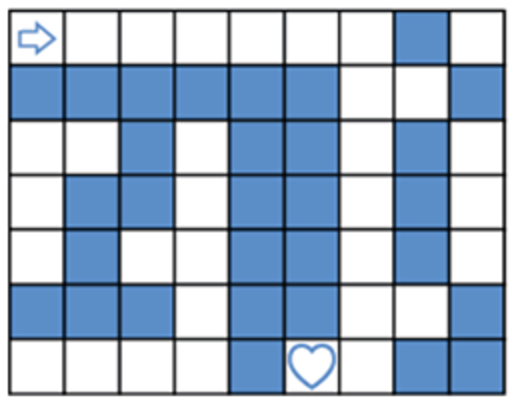
\includegraphics[width=0.5\linewidth]{images/move-robot.png}
    \caption{Quiz Question 9. Playtesters were asked to choose an algorithm that would move the arrow to the heart.}
    \label{fig:question-9}
\end{figure}

\subsection{Unity}
Unity has been a staple of the game development industry for both independent and first-party games alike since its release in 2005 \cite{unity-website}. This engine was my introduction to both game design and programming, as it is for many aspiring game developers due to its wealth of tutorials, documentation, and the fact that using the vast majority of its features is free. However, in September 2023, Unity announced a change to its pricing plans: developers whose games received over a certain number installs would suddenly be charged a fee for each subsequent download \cite{unity-deleted-post}. This choice was received as an attempt to exploit Unity’s long-time user base of game developers, and garnered notable backlash from players and developers alike. MegaCrit studios, the developers behind the highly successful Slay the Spire (2017), released a statement which noted their frustration with Unity’s changes and a removal of their Terms of Service from GitHub, and simultaneously announced that their new project would be migrating to an alternate, open source engine \cite{sts-tweet}. Despite Unity’s attempt to apologize and revert the decision to charge for installs \cite{unity-runtime-pricing}, they severely damaged their reputation.

Though the public opinion of Unity has shifted over the last year, it remains true that the reversion and alteration of the install fee policy ensured that independent and aspiring developers such as myself would not be impacted. Using Unity to develop a small-scale project that I plan to release for free would therefore not be unethical, though greater concerns would arise if I were in any way financially supporting Unity or profiting from my game.

\subsection{Monetization}
\textit{Magicode} is available to download for free on Itch.io, and its source code is publicly accessible on GitHub. Many games today, especially those with a younger audience, are monetized in a manner that tricks players into spending money, having their data collected against their will, or otherwise being misdirected. These strategies are known as Dark Patterns \cite{dark-patterns-website}, \cite{dark-patterns-from-class}. It is not possible to intentionally or accidentally spend money on \textit{Magicode}, so continued play must be driven by motivation to learn and enjoyment of the mechanics rather than psychological tricks.

\subsection{Accessibility}
The core mechanics of my game involve drag-and-drop coding and strategic warrior placement, which require the use of a mouse and keyboard. Lack of control accessibility is a common concern among players of all games \cite{ground-floor-accessibility}, and building a game that necessarily requires the use of fine motor skills also suggests the inclusion of accessibility options. Unfortunately, due to time constraints, \textit{Magicode} does not include alternate control schemes or other accessibility features. However, future work would include controller support, allowing a cursor to be moved around the screen with a joystick. Given that the game contains a sizable amount of informative text to be read, future work would also include voice acting and audio descriptions to assist players.

\subsection{Schooling and Students}
The American schooling system is founded on the basis of colonial ideologies that are inherently unethical and harmful to those it seeks to educate. I use the term “schooling” in place of “education” to intentionally draw a distinction between what it means to learn and what happens in the standardized classroom space. David Stovall \cite{stovall-abolition} uses this terminology in his article “Are We Ready for ‘School’ Abolition? Thoughts and Practices of Radical Imaginary in Education”, which explores the harmful nature of schooling, and how a new system of education founded in liberation is needed. What it means to be a “good” student or a “good” teacher is defined by how well one is able to operate within the system, where the process of learning is often defined by obedience to authority and rote memorization. In line with radical education practices, the goal is for my game to be supplemental: useful as a learning tool in the classroom, and fun enough that students would want to continue playing and learning in their own time.


\section{Conclusion}
\textit{Magicode} is an educational autobattler video game designed to teach the fundamentals of programming. Players enjoyed its approachability and the ways in which it simplified coding concepts that are often difficult to beginners. Strategy, difficulty, and effective level design all contributed to an enjoyable gameplay experience. Based on feedback, future development would include developing additional quality-of-life features to enhance the educational experience. This could take the form of additional instructional clarity through optional hints, a glossary reference for key terms, and additional levels that allow more time to be spent learning with each new mechanic.




% ~\\~\\

\sloppy
\printbibliography


\newpage

\appendix

\section{Appendix: Replication Instructions}
This project was built in Unity v2022.3.50f1 using the C\# language. To run the game, download the executable file from the \href{https://github.com/slevy14/Comps-Game/releases/tag/Release}{releases tab} of the GitHub repository where you found this paper, or from \href{https://leafguy.itch.io/magicode}{Itch.io}. To open the game in Unity, first download the correct version of the game editor from \href{https://unity.com/releases/2022-lts}{Unity's Website}. Next, download or clone this project's git repository, and open the folder entitled ``Comps Game'' through Unity's launch screen.

\section{Appendix: Code Architecture}
A wide array of scripts, scriptable objects, and Unity game objects are used across 5 different scene environments, though the game’s core functionality is summarized in Figure \ref{fig:architecture-diagram}, showing how the player regularly interacts with core game functionality. This is split between the code editor scripts and the battlefield scripts, with the list of all warriors stored in a persistent game object accessible in all scenes.

In the code editor, all player actions interface directly with the Designer Controller. This script is responsible for instantiating new code blocks, connecting code blocks to each other visually and in a linked list, and saving warrior data to an external file. The Draggable script stores references to connected blocks and allows players to drag and drop all blocks in the scene.

When loading the battlefield scene, the warrior list is referenced to create icons of all warriors that the player can drag and drop onto the battlefield, making use of the Placement System script. Dragging a new warrior to the battlefield instantiates a new warrior game object containing the Warrior Behavior script, storing saved property data and behavior lists from the persistent warrior list to the individual warrior. Interacting directly with a warrior displays their stats to the player and updates the list of all objects on the battlefield. When the player starts the battle, the Level Controller script sorts all warriors on the battlefield into a list organized by the speed stat, and loops through this list using all saved Move and UseWeapon functions on each warrior in order until the battle is either won or lost.

\begin{figure}
    \centering
    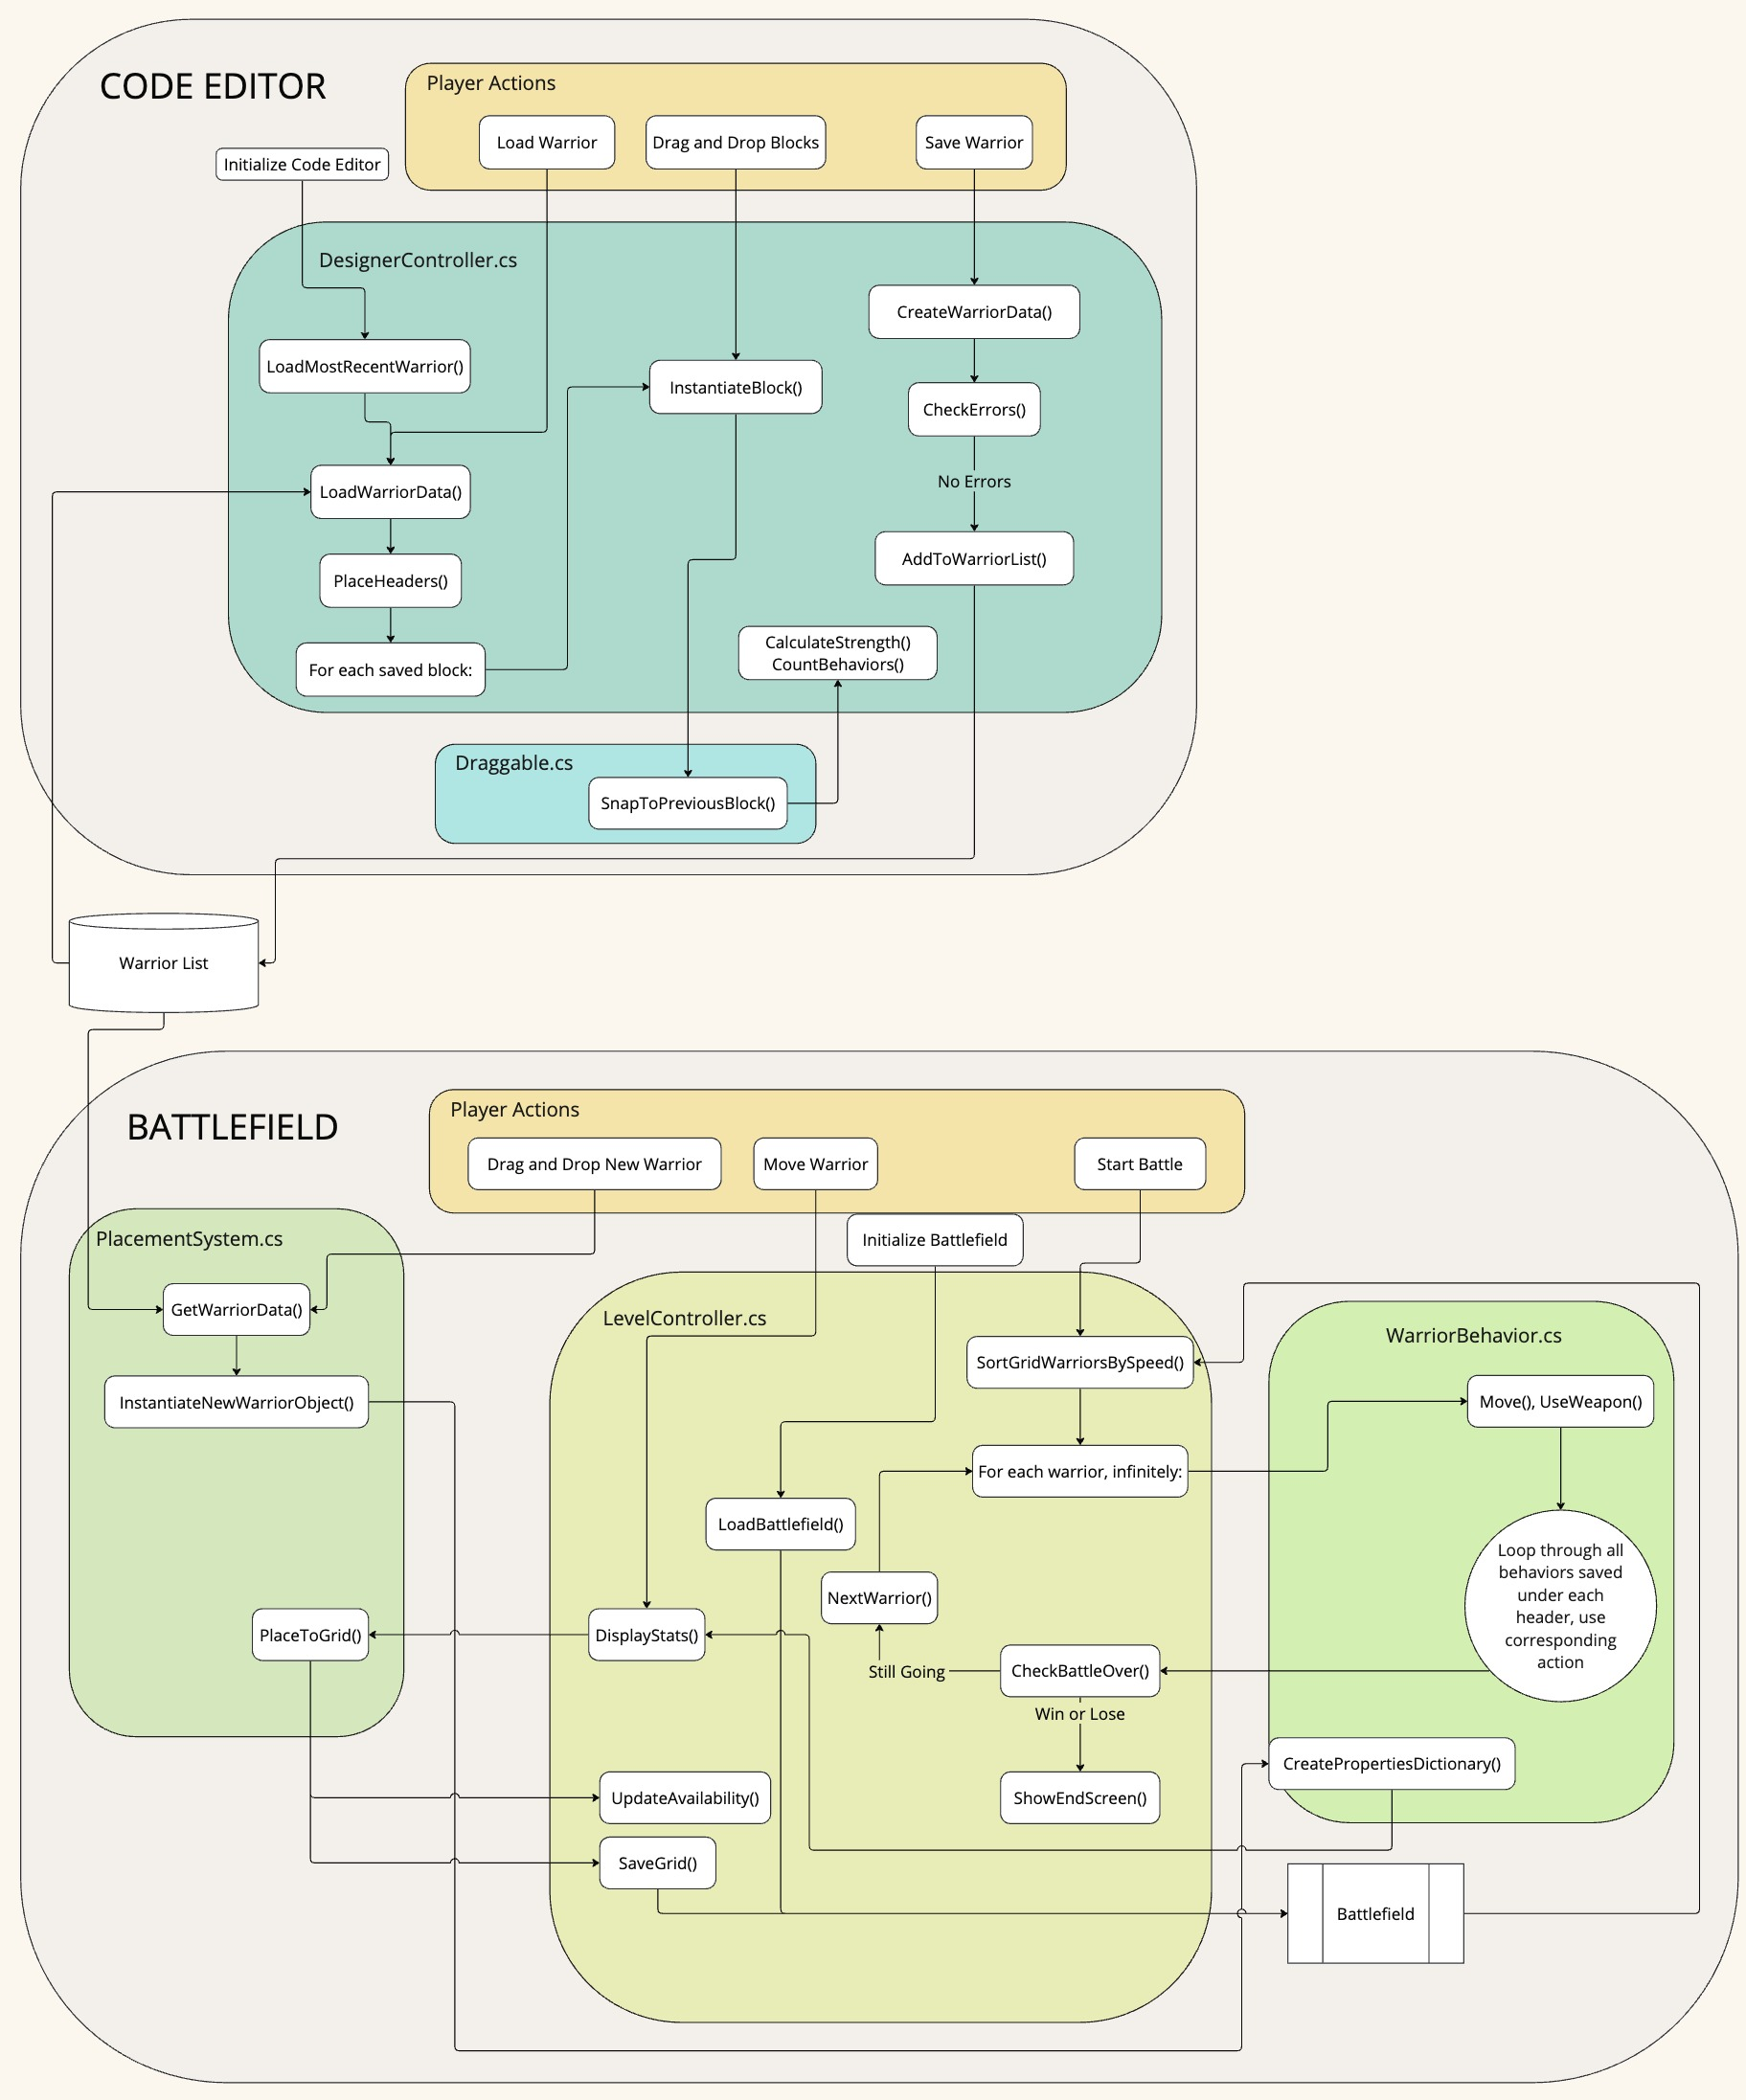
\includegraphics[width=\linewidth]{images/architecture-diagram.jpg}
    \caption{Code architecture diagram.}
    \label{fig:architecture-diagram}
\end{figure}

\end{document}

